% Slide thuyết trình CS331 (bản 2, 23/11/2026; sửa câu chữ + thuật ngữ 24/11) — biên dịch: latexmk -xelatex main.tex
% Kịch bản nói: latexmk -xelatex notes.tex (cùng nội dung, in phần \note của từng slide)
\documentclass[aspectratio=169,10pt]{beamer}
\usetheme[progressbar=frametitle,numbering=none,sectionpage=progressbar]{metropolis}
\ifdefined\withnotes
  \setbeameroption{show only notes}
  \setbeamerfont{note page}{size=\large}
\fi

\usepackage{fontspec}
\usepackage[vietnamese]{babel}
\setsansfont{TeX Gyre Heros}
\setmainfont{TeX Gyre Heros}
\usepackage{unicode-math}
\setmathfont{TeX Gyre Termes Math}
\usepackage{booktabs,array,tabularx,multirow}
\usepackage{pifont}
\usepackage{tikz}
\usetikzlibrary{positioning,arrows.meta,calc}
\graphicspath{{../../reports/figures/}{../shared/figures/}}
% Shared notation for report and slides (CS331).
\newcommand{\Bzero}{\textsf{B0}}
\newcommand{\Btwo}{\textsf{B2}}
\newcommand{\Pv}{\textsf{P}}
\newcommand{\Fv}{\textsf{F}}
\newcommand{\Tv}{\textsf{T}}
\newcommand{\Sv}{\textsf{S}}
\newcommand{\Csix}{\textsf{C6}}
\newcommand{\PF}{\textsf{P+F}}
\newcommand{\BtwoF}{\textsf{B2+F}}
\newcommand{\cgdpp}{CountGD++}
\newcommand{\MAE}{\mathrm{MAE}}
\newcommand{\RMSE}{\mathrm{RMSE}}
\newcommand{\FPRabs}{\mathrm{FPR}_{\text{absent}}}
\newcommand{\ci}[2]{\,[#1;\ #2]}
\newcommand{\todo}[1]{\textcolor{red}{[TODO: #1]}}
% Colours used by the TikZ figures
\definecolor{accent}{HTML}{1F5FA8}
\definecolor{good}{HTML}{1E8449}
\definecolor{bad}{HTML}{C0392B}
\definecolor{softgray}{HTML}{6B7280}
\definecolor{boxblue}{HTML}{DCE9F6}
\definecolor{boxorange}{HTML}{FDE6D2}
\definecolor{boxyellow}{HTML}{FFF3C4}
\definecolor{boxgreen}{HTML}{DAF0D5}
\definecolor{boxgray}{HTML}{F1F1F1}


% ---------------------------------------------------------------- look
\setbeamercolor{frametitle}{bg=accent!92!black,fg=white}
\setbeamercolor{progress bar}{fg=good,bg=accent!25}
\setbeamercolor{alerted text}{fg=bad}
\setbeamercolor{example text}{fg=good}
\setbeamercolor{normal text}{fg=black!88,bg=white}
\setbeamercolor{block title}{bg=accent!12,fg=accent!70!black}
\setbeamercolor{block body}{bg=accent!4}
\setbeamercolor{block title alerted}{bg=bad!12,fg=bad!80!black}
\setbeamercolor{block body alerted}{bg=bad!4}
\setbeamercolor{block title example}{bg=good!12,fg=good!70!black}
\setbeamercolor{block body example}{bg=good!4}
\metroset{block=fill}
\setbeamerfont{frametitle}{size=\normalsize,series=\bfseries}
\setbeamerfont{block title}{size=\small,series=\bfseries}
\setbeamertemplate{itemize items}{\textcolor{accent}{\small$\blacktriangleright$}}
\setlength{\leftmargini}{1.2em}

% Source line + page number in the footline (phân công công việc: slide 3)
\gdef\currentsource{}
\newcommand{\source}[1]{\gdef\currentsource{#1}}
\AtBeginEnvironment{frame}{\gdef\currentsource{}}
\setbeamertemplate{footline}{%
  \begin{beamercolorbox}[wd=\paperwidth,ht=4.2mm,dp=1.8mm,leftskip=3mm,rightskip=3mm]{footline}%
    {\tiny\color{softgray}\currentsource}%
    \hfill{\tiny\color{softgray}\insertframenumber/\inserttotalframenumber}%
  \end{beamercolorbox}}

\tikzset{
  sb/.style={draw=black!55,rounded corners=2pt,fill=#1,align=center,minimum height=10mm,inner sep=3pt,font=\sffamily\scriptsize},
  sa/.style={-{Stealth[length=1.8mm]},thick,black!70}}

\newcommand{\bignum}[1]{{\Large\bfseries\color{accent}#1}}
\newcommand{\takeaway}[1]{\par\vspace{1.5mm}{\centering\colorbox{accent!10}{\parbox{0.94\linewidth}{\centering\small\bfseries\color{accent!75!black}#1}}\par}}

\title{Đếm đúng class trong ảnh nhiều class:\\chẩn đoán và giảm lỗi ``đếm nhầm class'' của CountGD++}
\subtitle{Diagnosing and reducing class confusion of CountGD++ in multi-class images}
\author{Đào Xuân Minh Trí -- 24521826 \qquad Trần Đăng Khắc Triệu -- 24521857}
\institute{Trường Đại học Công nghệ Thông tin -- ĐHQG-HCM \quad·\quad Khoa Khoa học Máy tính\\[1mm]
Môn: Thị giác máy tính nâng cao (CS331) \quad·\quad GVHD: TS. Mai Tiến Dũng}
\date{}

\begin{document}

% ================================================================ Title
\begin{frame}
\titlepage
\note{[0:20] Chào thầy và các bạn. Nhóm em gồm Trí và Triệu. Đề tài của nhóm: kiểm tra xem CountGD++, một mô hình đếm theo text prompt, có đếm đúng class được hỏi khi trong ảnh có nhiều class hay không, và tìm cách giảm lỗi đếm nhầm.}
\end{frame}

\begin{frame}{Nội dung}
\setbeamertemplate{section in toc}[sections numbered]
\tableofcontents
\note{[0:15] Bài trình bày gồm năm phần: lý do chọn đề tài, bài toán, phương pháp, thực nghiệm, và cuối cùng là giới hạn, kết luận.}
\end{frame}

\begin{frame}{Phân công công việc}
\scriptsize\centering
\renewcommand{\arraystretch}{1.2}
\begin{tabularx}{\textwidth}{@{}>{\bfseries}p{0.17\textwidth} >{\raggedright\arraybackslash}X >{\raggedright\arraybackslash}X@{}}
\toprule
\normalfont\bfseries Hạng mục & \textbf{Trí} & \textbf{Triệu}\\
\midrule
Môi trường, baseline & Dựng CountGD++ trên Kaggle T4, chạy lại benchmark FSCD-147 (MAE 8.34) & Kiểm chéo evaluator, tính tay, self-test\\
Pilot, cải tiến v1 & Chạy pilot 5 ảnh, xem từng query bằng mắt; làm bộ lọc v1 & Tự kiểm lại kết quả v1\\
Chẩn đoán & Phân tích điểm theo token; quyết định thêm phép thử T trước khi khóa cấu hình & \textbf{Blind review 117 box (N4)}; phát hiện cơ chế max khi rà soát N4\\
Hướng cải tiến v2 & Chốt các quyết định D1--D10, chọn hướng P + T & \textbf{Đề xuất nhánh P}; chuẩn bị runner P, chạy pilot P trên T4\\
Dữ liệu & Kiểm 20 ảnh dev & Rút dev/test bằng script; \textbf{kiểm 40 ảnh test}; khóa dữ liệu\\
Thực nghiệm & Chọn và \textbf{khóa cấu hình} (freeze v2) & \textbf{Chạy dev, chạy test một lần}, chạy khảo sát FSC-147\\
Viết, trình bày & Bản báo cáo chi tiết, bản gửi thầy, báo cáo LaTeX, slide & Related Work, điểm yếu và hướng thử thêm, rà sửa slide\\
\bottomrule
\end{tabularx}
\note{[0:20] Đây là phân công công việc trong đồ án. Trí dựng môi trường, chạy pilot, làm cải tiến v1, chốt các quyết định và khóa cấu hình. Triệu làm blind review, đề xuất nhánh P, rút và kiểm dữ liệu test, chạy dev, test và khảo sát FSC-147.}
\end{frame}

% ================================================================ 1
\section{Lý do thực hiện đề tài}

\begin{frame}{Bối cảnh: đếm vật chỉ bằng tên class}
\source{Ranjan và cs., CVPR 2021; Amini-Naieni \& Zisserman, CVPR 2026}
\begin{columns}[T]
\begin{column}{0.54\textwidth}
\begin{itemize}
\item \textbf{Class-agnostic counting}: class cần đếm được chỉ định lúc dùng, không phải huấn luyện riêng cho từng class
\item Chỉ định bằng exemplar box, hoặc chỉ bằng \textbf{text prompt} (zero-shot, text-only); thực tế người dùng thường chỉ có tên class
\item \textbf{CountGD++} (CVPR 2026): mô hình đếm theo text prompt mạnh hiện nay, tự chọn \emph{pseudo-exemplar} lúc suy luận
\end{itemize}
\end{column}
\begin{column}{0.42\textwidth}
\begin{block}{Kiểm tra môi trường (FSCD-147 test, 1.190 ảnh)}
\centering\small
\begin{tabular}{@{}lrr@{}}
\toprule
& MAE $\downarrow$ & RMSE $\downarrow$\\
\midrule
Bài báo (Ours t+p+s) & 8.39 & 27.03\\
Nhóm chạy lại & \textbf{8.34} & \textbf{24.64}\\
\bottomrule
\end{tabular}\\[1mm]
{\scriptsize Cùng checkpoint công khai $\Rightarrow$ môi trường chạy đúng; đây không phải cải tiến của nhóm.}
\end{block}
\end{column}
\end{columns}
\takeaway{Câu hỏi: chỉ với tên class, mô hình có đếm \emph{đúng class được hỏi} không?}
\note{[0:50] Đếm vật có nhiều ứng dụng. Hướng hiện đại cho phép chỉ định class cần đếm ngay lúc dùng, kể cả chỉ bằng tên class. Nhóm chọn CountGD++, công bố ở CVPR 2026. Trước tiên nhóm chạy lại benchmark của bài báo, được MAE 8.34 so với 8.39, nên môi trường chạy đúng.}
\end{frame}

\begin{frame}{Khoảng trống: benchmark quen thuộc không kiểm tra việc đếm đúng class}
\source{Ciampi và cs., WACV 2025 (PrACo); Pacini và cs., 2026 (MUCCA)}
\begin{columns}[T]
\begin{column}{0.48\textwidth}
\begin{alertblock}{FSC-147: mỗi ảnh chỉ có một class nổi bật}
\begin{itemize}\small
\item Class được hỏi luôn có trong ảnh
\item Chỉ cần đếm vật nổi bật nhất là đã đạt điểm cao
\item PrACo: mô hình mạnh vẫn đếm ra số khi hỏi class \emph{không có} trong ảnh
\end{itemize}
\end{alertblock}
\end{column}
\begin{column}{0.48\textwidth}
\begin{exampleblock}{MUCCA (2026): ảnh thật, nhiều class}
\begin{itemize}\small
\item 200 ảnh, 45 class, có \textbf{nhãn điểm cho từng class} trong cùng ảnh
\item Đo được: hỏi X có đếm nhầm sang Y không; hỏi class vắng mặt có trả 0 không
\end{itemize}
\end{exampleblock}
\end{column}
\end{columns}
\vspace{2mm}
\begin{block}{Bài toán X/Y (theo câu hỏi của giảng viên)}
\small Cùng một ảnh có X và Y: hỏi X thì đếm X; đổi sang Y thì đếm Y và \textbf{không đếm lại X}; hỏi Z không có trong ảnh thì phải trả \textbf{0}.
\end{block}
\note{[0:50] Benchmark chuẩn FSC-147 gần như ảnh nào cũng chỉ có một class, nên không kiểm được việc đếm đúng class. PrACo đã chỉ ra mô hình vẫn đếm ra số khi hỏi class không có trong ảnh. MUCCA là bộ ảnh thật năm 2026, có nhãn cho nhiều class trong cùng ảnh, nên kiểm được đúng bài X/Y.}
\end{frame}

\begin{frame}{Related work và vị trí của đồ án}
\source{Huang và cs., CVPR 2024; Pelhan và cs., CVPR 2024; Zhu và cs., ECCV 2024}
\footnotesize
\renewcommand{\arraystretch}{1.1}
\begin{tabularx}{\textwidth}{@{}l >{\raggedright\arraybackslash}X c l@{}}
\toprule
Công trình & Ý chính & Huấn luyện? & Liên hệ\\
\midrule
CountGD / CountGD++ & Đếm theo text prompt trên nền Grounding DINO; pseudo-exemplar hai lượt & có & mô hình gốc\\
PseCo & SAM đề xuất vùng, classifier CLIP được distill & có & \\
VA-Count & Tìm exemplar tốt, contrastive learning loại exemplar xấu & có & gần bước \textbf{P}\\
DAVE & Detect rồi verify; bản text prompt dùng CLIP loại cả \emph{cụm} box & có & gần bước \textbf{F}\\
PrACo, MUCCA & Đo mức bám prompt (class vắng mặt, vật gây nhiễu) & không & cách đánh giá\\
\midrule
\textbf{Đồ án} & Chẩn đoán lỗi trên ảnh nhiều class; CLIP kiểm \textbf{từng box}; giao thức khóa trước & \textbf{không} & \\
\bottomrule
\end{tabularx}
\takeaway{Không huấn luyện mô hình mới, cũng không chỉ đánh giá: nhóm sửa ở bước suy luận của mô hình có sẵn.}
\note{[0:45] Các phương pháp tự tạo exemplar như PseCo, VA-Count, DAVE đều phải huấn luyện thêm. Gần nhất với bước lọc F là bản dùng text prompt của DAVE, nhưng DAVE loại theo cụm box và có huấn luyện; F kiểm từng box và không huấn luyện. PrACo và MUCCA chỉ đánh giá. Đồ án nằm giữa: chẩn đoán và sửa ở bước suy luận.}
\end{frame}

% ================================================================ 2
\section{Mô tả bài toán}

\begin{frame}{Định nghĩa: input, output và ba yêu cầu}
\begin{columns}[T]
\begin{column}{0.50\textwidth}
\textbf{Input:} ảnh $I$ và tên class $t$ (chỉ text, không có exemplar)\\[1mm]
\textbf{Output:} số đếm $\hat n(I,t)\in\mathbb{N}$ và tập box $B(I,t)$\\[1mm]
\textbf{Nhãn:} $\mathcal{C}(I)$ là tập class có trong ảnh, $n_c(I)$ là số vật của class $c$\\[2mm]
\textbf{Mỗi ảnh đánh giá có 3 query:}
\begin{itemize}\small
\item 2 \textbf{present query}: X, Y $\in\mathcal{C}(I)$
\item 1 \textbf{absent query} Z, chọn khó (cùng nhóm nghĩa với Y), người kiểm xác nhận không có trong ảnh
\end{itemize}
\end{column}
\begin{column}{0.46\textwidth}
\begin{block}{Ba yêu cầu}
\small
\textbf{(Y1)} $t\in\mathcal{C}(I)\Rightarrow \hat n(I,t)\approx n_t(I)$\\[1.5mm]
\textbf{(Y2)} $t\notin\mathcal{C}(I)\Rightarrow \hat n(I,t)=0$\\[1.5mm]
\textbf{(Y3)} $X\neq Y \Rightarrow B(I,X)$ và $B(I,Y)$ \textbf{khác nhau}: mỗi box chỉ thuộc đúng class được hỏi
\end{block}
\end{column}
\end{columns}
\note{[0:50] Input là ảnh và tên class, không có exemplar. Output là số đếm và các box. Mỗi ảnh có hai present query X, Y và một absent query Z, được chọn khó, cùng nhóm nghĩa. Ba yêu cầu: đếm đúng khi class có mặt, trả 0 khi vắng mặt, và đổi query thì tập box cũng phải đổi.}
\end{frame}

\begin{frame}{Minh họa: ba query khác nhau, gần như cùng một tập box}
\source{Ảnh MUCCA mcac\_12 (test). Box của CountGD++ hai lượt (\Btwo), lấy từ dự đoán đã lưu}
\centering
\begin{tabular}{@{}c@{\hspace{2mm}}c@{\hspace{2mm}}c@{}}
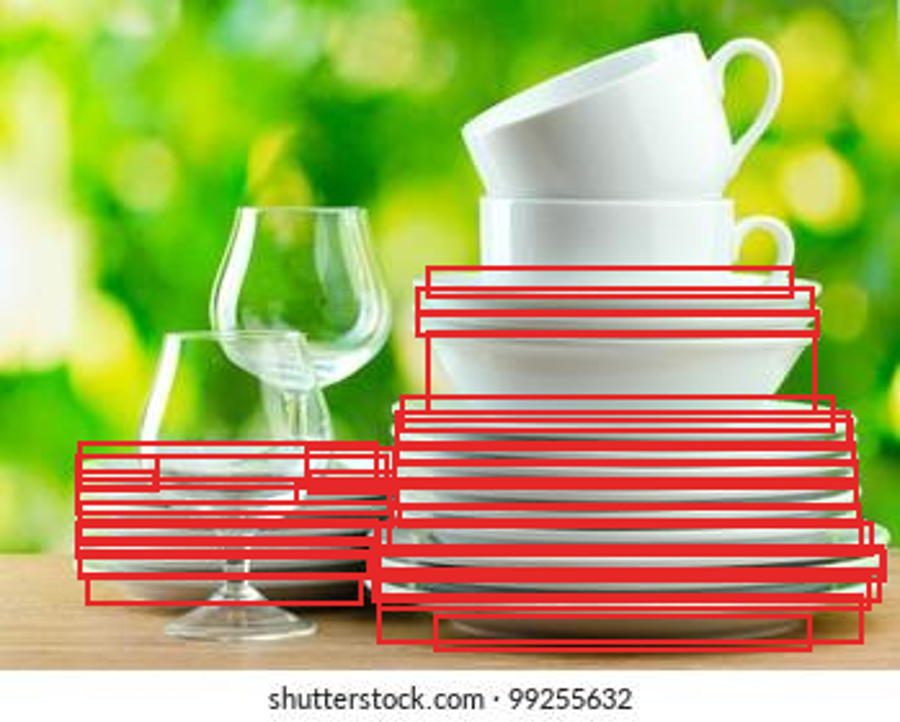
\includegraphics[width=0.31\textwidth]{xy_mcac12_B2_t01_1.png} &
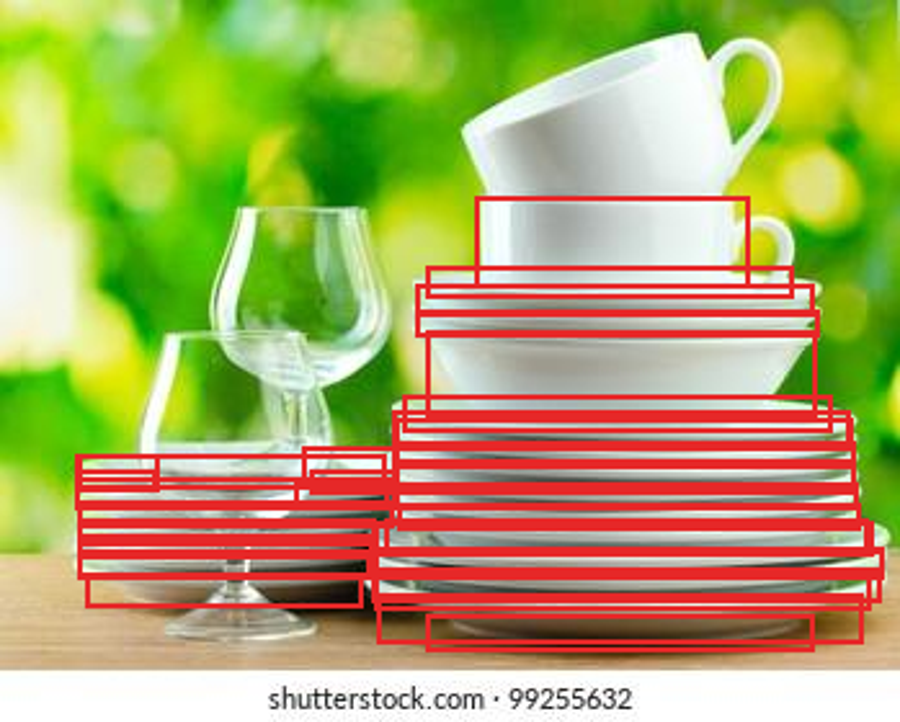
\includegraphics[width=0.31\textwidth]{xy_mcac12_B2_t01_2.png} &
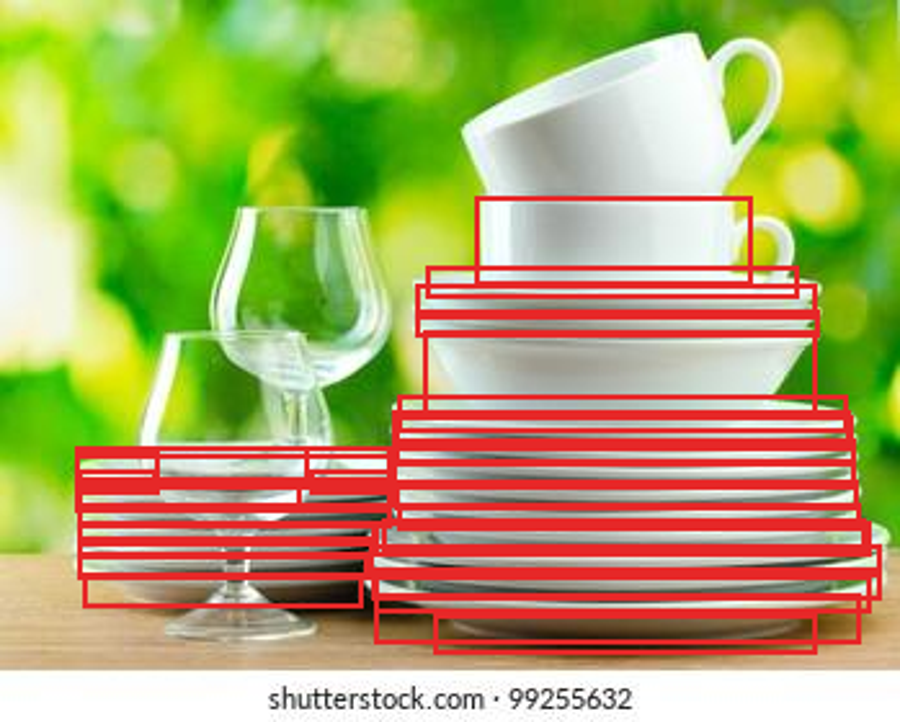
\includegraphics[width=0.31\textwidth]{xy_mcac12_B2_t01_3.png}\\
\small X = ``plates'': đếm \alert{36} (GT 16) &
\small Y = ``bowls'': đếm \alert{36} (GT 3) &
\small Z = ``spoons'': đếm \alert{34} (GT 0)
\end{tabular}
\takeaway{36/36 box của query ``plates'' cũng xuất hiện ở query ``bowls'' (IoU $\ge 0.5$): đổi query, mô hình gần như không đổi box.}
\note{[0:50] Đây là ví dụ thật trên tập test. Ảnh có đĩa, bát, cốc và ly. Hỏi plates, GT là 16; hỏi bowls, GT là 3; hỏi spoons, không có trong ảnh, GT là 0. CountGD++ trả 36, 36 và 34, và cả 36 box của query plates đều xuất hiện lại ở query bowls. Đây chính là lỗi X/Y.}
\end{frame}

\begin{frame}{Câu hỏi nghiên cứu và đóng góp}
\begin{columns}[T]
\begin{column}{0.32\textwidth}
\begin{block}{RQ1 · Chẩn đoán}
\small \cgdpp{} sai ở đâu trên ảnh nhiều class? Lỗi đến từ bước nào?
\end{block}
\end{column}
\begin{column}{0.32\textwidth}
\begin{block}{RQ2 · Cải tiến}
\small Có giảm được lỗi mà \textbf{không huấn luyện lại} không?
\end{block}
\end{column}
\begin{column}{0.32\textwidth}
\begin{block}{RQ3 · Kiểm chứng}
\small Mức cải thiện có giữ được trên ảnh \textbf{chưa từng dùng}, khi cấu hình đã khóa trước không?
\end{block}
\end{column}
\end{columns}
\vspace{3mm}
\textbf{Đóng góp}
\begin{enumerate}\small
\item Chẩn đoán bằng số đo: shared box X/Y, pseudo-exemplar sai class, phần lỗi do phép $\max$ (biến thể T)
\item Hai bước dùng CLIP, không huấn luyện: kiểm pseudo-exemplar (\Pv) và lọc box (\Fv), mỗi bước có đối chứng riêng
\item Giao thức ``chọn trước, xem sau'': dữ liệu khóa, luật chọn viết trước, test chạy một lần
\item Báo cáo cả kết quả âm và phạm vi áp dụng
\end{enumerate}
\note{[0:40] Ba câu hỏi: mô hình sai ở đâu, có sửa được mà không huấn luyện lại không, và mức sửa có còn giữ trên ảnh chưa từng dùng không. Bốn đóng góp như trên slide. Chuyển: em mời thầy xem CountGD++ đếm như thế nào.}
\end{frame}

% ================================================================ 3
\section{Phương pháp}

\begin{frame}{Baseline CountGD++: một lượt (\Bzero) và hai lượt (\Btwo)}
\source{Amini-Naieni \& Zisserman, CVPR 2026; mã \texttt{CountGDPlusPlus/process\_folder.py}}
\begin{center}
\begin{tikzpicture}[node distance=5mm]
\node[sb=boxgray] (i) {Ảnh +\\``bowls .''};
\node[sb=boxblue,right=of i] (l1) {\textbf{Lượt 1}\\900 box đề xuất};
\node[sb=boxgray,right=of l1] (t) {Giữ box\\$s(b)>0.23$};
\node[sb=boxorange,right=of t] (m) {Top-3 box\\= \textbf{pseudo-exemplar}};
\node[sb=boxblue,right=of m] (l2) {\textbf{Lượt 2}\\text + pseudo-exemplar};
\node[sb=boxgray,right=of l2] (o) {Số đếm =\\số box $>0.23$};
\draw[sa] (i)--(l1); \draw[sa] (l1)--(t); \draw[sa] (t)--(m); \draw[sa] (m)--(l2); \draw[sa] (l2)--(o);
\node[font=\scriptsize\bfseries,text=accent,below=1mm of t] {\Bzero{} dừng ở đây};
\end{tikzpicture}
\end{center}
\begin{columns}[T]
\begin{column}{0.50\textwidth}
\textbf{Điểm của một box}
\[ s(b)=\max_{k\,\in\,\text{token trước dấu chấm}} s_k(b) \]
{\small Ở lượt 2, mỗi pseudo-exemplar thêm một token, nên phép $\max$ xét cả text token lẫn exemplar token.}
\end{column}
\begin{column}{0.46\textwidth}
\begin{block}{Hình dung}
\small Người đếm chỉ vào 3 vật mình chắc nhất rồi nói: ``đếm hết những thứ trông như thế này''. Nếu 3 vật đó \alert{sai class}, lượt 2 sẽ sai một cách rất tự tin.
\end{block}
{\scriptsize Dùng checkpoint công khai, không huấn luyện lại. Lượt 1 không có box nào thì \Btwo{} trả kết quả của \Bzero.}
\end{column}
\end{columns}
\note{[1:00] Ở lượt 1, mô hình đọc text prompt và chấm điểm 900 box; box nào trên 0.23 thì được đếm. Đó là B0. Lượt 2 lấy 3 box chắc nhất làm pseudo-exemplar rồi chạy lại; đó là chế độ hai lượt B2. Điểm của một box là max qua các token, và ở lượt 2 có thêm cả exemplar token. Chuyển: phần chẩn đoán, bạn Triệu trình bày.}
\end{frame}

\begin{frame}{Chẩn đoán: ba vấn đề và hướng xử lý}
\footnotesize
\renewcommand{\arraystretch}{1.15}
\begin{tabularx}{\textwidth}{@{}>{\raggedright\arraybackslash}p{0.20\textwidth} >{\raggedright\arraybackslash}X >{\raggedright\arraybackslash}p{0.21\textwidth} >{\raggedright\arraybackslash}p{0.22\textwidth}@{}}
\toprule
Vấn đề & Bằng chứng & Nguyên nhân (giả thuyết) & Hướng xử lý\\
\midrule
\textbf{VĐ1.} Đổi query, box gần như không đổi & Test: 64\% box là shared box giữa query X và Y. Ảnh mcac\_88: cả 21 box ``people'' trùng box ``cars'' & Mô hình bám vào vật nổi bật trong ảnh hơn là bám vào prompt & \textbf{Filter F}: CLIP kiểm từng box theo đúng prompt\\
\textbf{VĐ2.} Pseudo-exemplar hay chọn nhầm class & Blind review: chỉ 1/12 pseudo-exemplar đúng class (present query) & Lấy 3 box điểm cao nhất, không kiểm class & \textbf{P}: CLIP kiểm pseudo-exemplar trước lượt 2\\
\textbf{VĐ3.} Lượt 2 làm lỗi nặng thêm & \Btwo{} kém \Bzero{} ở cả pilot, p4 và test & Điểm lượt 2 $=\max(\text{text score},\text{exemplar score})$ & \textbf{T}: chỉ chấm bằng text score (để kiểm giả thuyết)\\
\bottomrule
\end{tabularx}
\takeaway{Mỗi vấn đề có số đo cụ thể; mỗi hướng xử lý được thử riêng để biết hướng nào thật sự có ích.}
\note{[0:45] Từ pilot, blind review và tập test, nhóm tách ra ba vấn đề. Một: đổi query mà box gần như không đổi. Hai: pseudo-exemplar hay chọn nhầm class. Ba: lượt 2 làm lỗi nặng thêm vì cách chấm max. Mỗi vấn đề có một hướng xử lý, và nhóm thử riêng từng hướng.}
\end{frame}

\begin{frame}{VĐ1: đổi query, mô hình vẫn khoanh những vật cũ}
\source{Ảnh mcac\_88 (tập p4\_unseen\_v1), chế độ \Btwo; số liệu test từ phân tích post-hoc trên 39 ảnh}
\centering
\begin{tabular}{@{}c@{\hspace{2mm}}c@{\hspace{2mm}}c@{}}
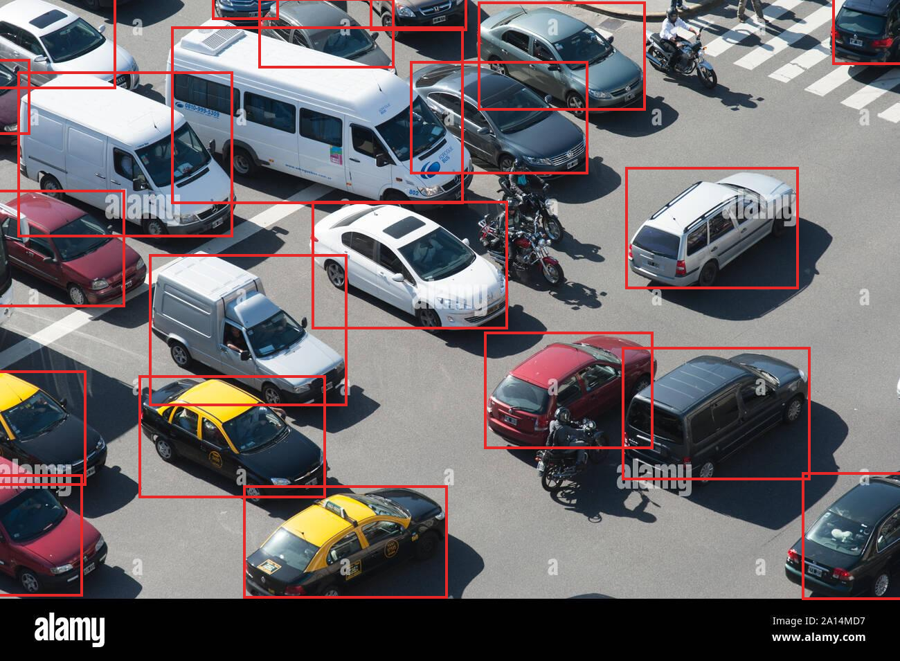
\includegraphics[width=0.24\textwidth]{xy_mcac88_B2_u07_1.png} &
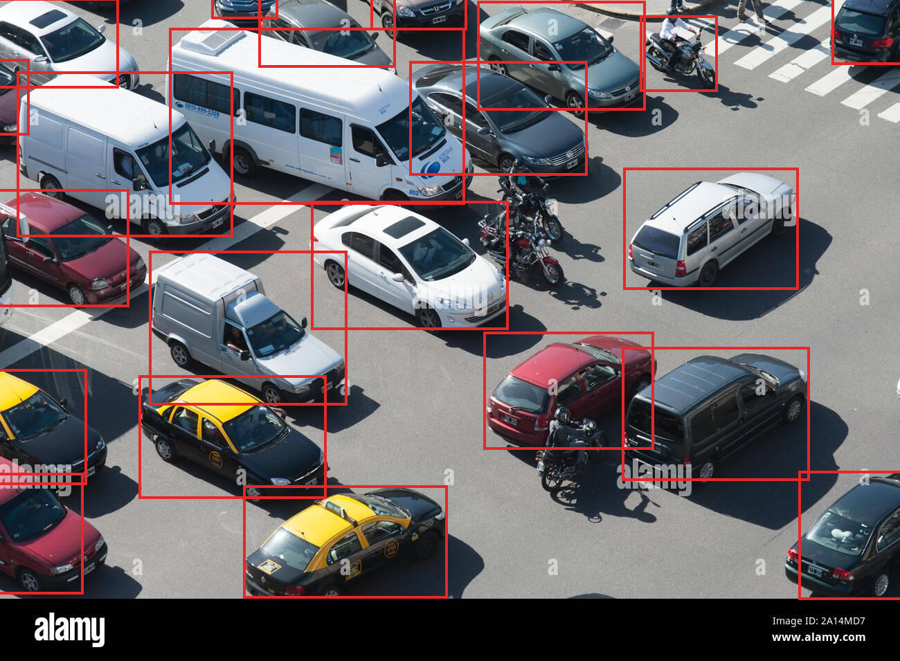
\includegraphics[width=0.24\textwidth]{xy_mcac88_B2_u07_2.png} &
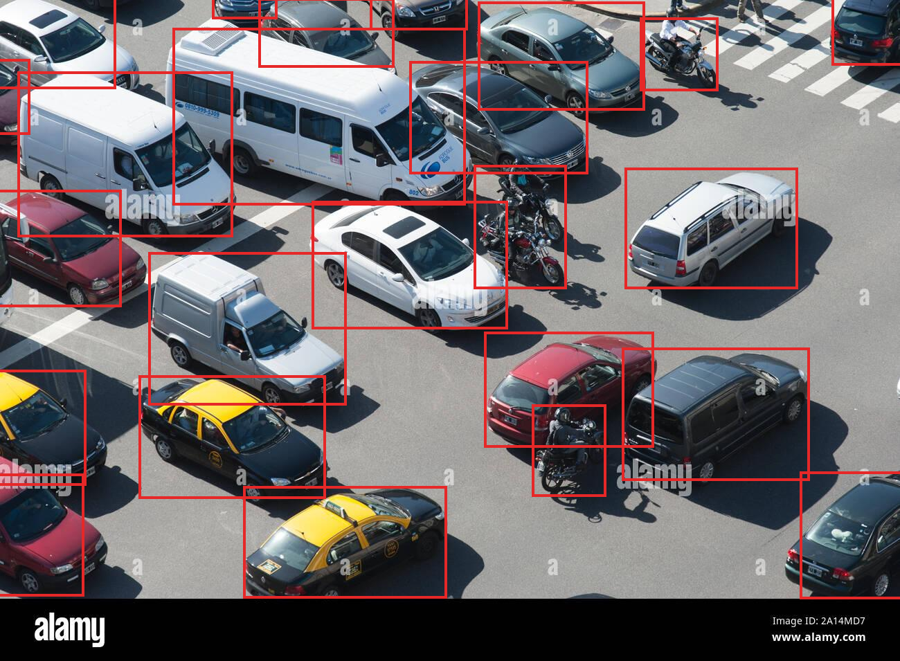
\includegraphics[width=0.24\textwidth]{xy_mcac88_B2_u07_3.png}\\
\scriptsize ``people'': \alert{21} (GT 6) & \scriptsize ``cars'': 22 (GT 22) & \scriptsize ``bicycles'': \alert{24} (GT 0)
\end{tabular}
\vspace{2mm}
\begin{columns}[T]
\begin{column}{0.47\textwidth}
\begin{itemize}\small
\item Cả 21 box của query ``people'' đều trùng với box của query ``cars'' (IoU $\ge 0.8$)
\item Hỏi ``people'' hay ``bicycles'' (ảnh không có xe đạp), mô hình vẫn khoanh chính những chiếc ô tô ấy
\end{itemize}
\end{column}
\begin{column}{0.47\textwidth}
\begin{itemize}\small
\item Trên tập test (\Bzero): \textbf{64\%} là shared box khi đổi query; \textbf{35\%} box nằm trên vật thuộc class khác
\item Với absent query, 92--100\% box đếm nhầm nằm trên một vật \emph{có thật} khác, không phải trên nền
\end{itemize}
\end{column}
\end{columns}
\note{[0:55] Ở ảnh này, hỏi people, cars hay bicycles thì mô hình đều khoanh gần như cùng những chiếc ô tô: cả 21 box của query people trùng với box của query cars. Trên tập test, đổi query thì 64 phần trăm box vẫn giữ nguyên, và khoảng một phần ba box nằm trên vật class khác. Khi hỏi class không có trong ảnh, box đếm nhầm gần như luôn nằm trên một vật có thật khác, không phải trên nền.}
\end{frame}

\begin{frame}{VĐ2: pseudo-exemplar thường rơi vào vật khác class}
\source{Blind review N4 (Triệu gán nhãn, Trí đối chiếu 9/9 box trùng); pilot 5 ảnh}
\begin{columns}[T]
\begin{column}{0.48\textwidth}
\textbf{Blind review 117 box ở 7 query bị lỗi}
\begin{center}\small
\begin{tabular}{@{}lr@{}}
\toprule
21 pseudo-exemplar & Số lượng\\
\midrule
Đúng class & \textbf{1}\\
Một box chứa nhiều vật & 10\\
Sai class & 10\\
\bottomrule
\end{tabular}
\end{center}
{\scriptsize Các query lỗi được chọn để phân tích, không đại diện cho cả tập. 9/21 pseudo-exemplar thuộc absent query (không thể đúng class); chỉ tính present query thì 1/12 đúng class.}
\end{column}
\begin{column}{0.48\textwidth}
\textbf{Pilot (5 ảnh, 15 present query)}
\begin{itemize}\small
\item 23/42 pseudo-exemplar đúng class
\item Query ``blackberries'' (GT 21): \Btwo{} đếm ra \alert{79}
\item MAE: \Bzero{} 19.4, \Btwo{} 22.0
\end{itemize}
\begin{block}{Hệ quả}
\small Pseudo-exemplar sai class $\Rightarrow$ lượt 2 đi tìm thêm những vật giống exemplar sai $\Rightarrow$ đếm thừa vật của class khác.
\end{block}
\end{column}
\end{columns}
\note{[0:50] Em blind review 117 box. Trong 21 pseudo-exemplar, chỉ 1 cái đúng class; 10 cái là một box chứa nhiều vật, 10 cái sai class. Cần lưu ý 9 trong 21 pseudo-exemplar thuộc absent query, vốn không thể đúng; chỉ tính present query thì 1 trên 12. Đây là các query lỗi được chọn để phân tích, không phải tỉ lệ chung của mô hình. Ở pilot cũng vậy: chỉ 23 trên 42 pseudo-exemplar đúng class, và có query blackberries GT 21 mà B2 đếm ra 79.}
\end{frame}

\begin{frame}{VĐ3: lượt 2 chấm điểm bằng $\max$, và phép thử \Tv}
\source{Dev v2 (20 ảnh) và p4\_unseen\_v1 (10 ảnh); CI 95\% bootstrap theo ảnh}
\begin{columns}[T]
\begin{column}{0.50\textwidth}
\[ s_{\text{lượt 2}}(b)=\max\bigl(\underbrace{s_{\text{text}}(b)}_{\text{giống ``people''?}},\ \underbrace{s_{\text{exemplar}}(b)}_{\text{giống exemplar?}}\bigr) \]
\textbf{Ví dụ đã lưu} (query ``people''): một box ô tô có text score $0.077$ nhưng exemplar score $0.970$ $\Rightarrow$ vẫn được giữ.\\[2mm]
\textbf{Giả thuyết H1:} lượt 2 gây hại là do phép $\max$.\\
\textbf{Phép thử \Tv:} vẫn chạy lượt 2 nhưng chỉ chấm bằng text score.
\end{column}
\begin{column}{0.46\textwidth}
\begin{center}\small
\begin{tabular}{@{}lrrr@{}}
\toprule
MAE $\downarrow$ & \Bzero & \Tv & \Btwo\\
\midrule
dev v2 & 6.28 & 8.55 & 9.15\\
p4\_unseen\_v1 & 6.77 & 8.80 & 13.00\\
\bottomrule
\end{tabular}
\end{center}
\begin{itemize}\small
\item \Tv{} chỉ gỡ được khoảng \textbf{21\%} tác hại trên dev (CI 95\% [5\%, 60\%])
\item \Tv{} vẫn kém \Bzero: $+2.27$ [$+0.52$, $+4.12$]
\end{itemize}
\begin{alertblock}{Kết luận}
\small Phép $\max$ chỉ giải thích \textbf{một phần}. Giả thuyết H2 (chưa kiểm): pseudo-exemplar làm lệch luôn cả text score.
\end{alertblock}
\end{column}
\end{columns}
\note{[1:00] Đọc mã thì thấy ở lượt 2, điểm của box là max giữa text score và exemplar score. Ví dụ đã lưu: một box ô tô có text score chỉ 0.077 nhưng exemplar score 0.97, nên vẫn được giữ khi hỏi people. Nhóm thử biến thể T bỏ phép max: T chỉ gỡ được khoảng một phần năm tác hại, và vẫn kém B0. Vậy max chỉ là một phần nguyên nhân; phần còn lại nhóm đặt giả thuyết H2, chưa kiểm. Chuyển: từ chẩn đoán này, Trí trình bày cách sửa.}
\end{frame}

\begin{frame}{Cải tiến P: CLIP kiểm pseudo-exemplar trước lượt 2}
\source{CLIP ViT-B/32 (Radford và cs., ICML 2021), revision cố định}
\begin{columns}[T]
\begin{column}{0.52\textwidth}
\begin{block}{Thuật toán P($\tau$, $M$)}
\small
\begin{enumerate}
\item Lấy $M$ box điểm cao nhất ở lượt 1
\item Crop từng box, tính $c=\cos\bigl(\text{CLIP}_{\text{image}}(\text{crop}),\ \text{CLIP}_{\text{text}}(\text{``a photo of }t\text{''})\bigr)$
\item Giữ các box có $c \ge \tau$; lấy tối đa 3 box theo điểm CountGD++
\item Không còn box nào $\Rightarrow$ trả kết quả \Bzero
\end{enumerate}
\end{block}
\end{column}
\begin{column}{0.44\textwidth}
\textbf{Ý tưởng:} sửa \emph{đầu vào} của lượt 2 (VĐ2), thay vì chỉ lọc ở cuối.\\[2mm]
\textbf{CLIP không đếm:} CLIP chỉ trả lời ``crop này có giống class được hỏi không''.\\[2mm]
\textbf{Tham số chọn trên dev:} $\tau\in\{0.18,\dots,0.28\}$, $M\in\{5,10\}$ $\Rightarrow$ khóa $\tau=0.20$, $M=5$.
\end{column}
\end{columns}
\note{[0:50] Cải tiến P nhắm vào vấn đề 2. Trước lượt 2, xét 5 box điểm cao nhất, dùng CLIP so crop của từng box với câu a photo of tên class, chỉ giữ những box đủ giống, rồi mới chọn pseudo-exemplar. Nếu không còn box nào thì trả kết quả một lượt.}
\end{frame}

\begin{frame}{Cải tiến F: lọc box bằng điểm kết hợp CountGD++ và CLIP}
\source{Query test t05\_1 (``blueberries'', ảnh có 5 loại quả); tham số khóa trong \texttt{freeze\_v2\_20261111.json}}
\begin{columns}[T]
\begin{column}{0.46\textwidth}
Với box $b$: điểm CountGD++ $a_b$, cosine CLIP $c_b$
\[ \tilde a_b=\mathrm{clip}\Bigl(\tfrac{a_b-a_{\min}}{a_{\max}-a_{\min}},0,1\Bigr),\ \ \tilde c_b \text{ tương tự} \]
\[ F_b=0.5\,\tilde a_b+0.5\,\tilde c_b \ \ge\ \theta \Rightarrow \text{giữ} \]
{\small Chọn trên dev rồi khóa: $a\in[0.231,0.982]$, $c\in[0.123,0.335]$, $\theta=0.604$.}
\end{column}
\begin{column}{0.50\textwidth}
\begin{center}\scriptsize
\begin{tabular}{@{}rrrrll@{}}
\toprule
\# & $a$ & $c$ & $F$ & Quyết định & Vật thật\\
\midrule
1 & 0.911 & 0.251 & \textbf{0.753} & giữ & việt quất \textcolor{good}{\ding{51}}\\
2 & 0.761 & 0.215 & 0.571 & bỏ & việt quất \textcolor{bad}{\ding{55}}\\
3 & 0.888 & 0.274 & 0.793 & giữ & quả khác \textcolor{bad}{\ding{55}}\\
4 & 0.727 & 0.218 & 0.554 & bỏ & không có vật \textcolor{good}{\ding{51}}\\
\bottomrule
\end{tabular}
\end{center}
{\small F bỏ được box không chứa vật, nhưng có thể bỏ nhầm vật đúng và giữ vật sai khi CLIP cũng nhầm.}
\end{column}
\end{columns}
\note{[0:55] Cải tiến F nhắm vào vấn đề 1. Mỗi box có điểm CountGD++ và điểm CLIP; đưa cả hai về khoảng 0 đến 1, lấy mỗi bên một nửa, và giữ box vượt threshold 0.604. Ví dụ thật: box không chứa vật bị bỏ, nhưng có một quả việt quất bị bỏ nhầm và một quả khác loại bị giữ nhầm.}
\end{frame}

\begin{frame}{Tổng thể: các biến thể được so sánh}
\centering
\resizebox{0.80\textwidth}{!}{% Pipeline cho slide (thuật ngữ tiếng Anh theo bảng thuật ngữ 24/11): B0, B2, P, F, C6.
% Bản cho báo cáo vẫn là pipeline.tex. Cần tikz libraries positioning, arrows.meta, calc; pifont.
\begin{tikzpicture}[
  font=\sffamily\footnotesize,
  node distance=6mm and 8mm,
  blk/.style={draw=black!70, rounded corners=2pt, align=center, minimum height=13mm, inner sep=3pt, line width=0.5pt},
  arr/.style={-{Stealth[length=2mm]}, line width=0.6pt, black!75},
  lab/.style={font=\sffamily\scriptsize, align=center}
]
\node[blk, fill=boxgray, text width=19mm] (in) {Ảnh + prompt\\(``bowls'')};
\node[blk, fill=boxblue, text width=24mm, right=of in] (s1) {\textbf{CountGD++ lượt 1}\\(chỉ text)};
\node[blk, fill=boxorange, text width=24mm, right=of s1] (ex) {Chọn pseudo-exemplar:\\top-3 box lượt 1};
\node[blk, fill=boxblue, text width=26mm, right=of ex] (s2) {\textbf{CountGD++ lượt 2}\\(text + pseudo-exemplar)};
\node[blk, fill=boxgreen, text width=28mm, right=of s2] (f) {\textbf{Filter F}\\$0.5\,\tilde a + 0.5\,\tilde c \ge \theta$};
\node[blk, fill=boxgray, text width=11mm, right=7mm of f] (out) {\textbf{Số đếm}};
\node[blk, fill=boxgray, text width=24mm, above=8mm of s1] (b0) {\textbf{B0}: số box\\có điểm $> 0.23$};
\node[blk, fill=boxyellow, text width=26mm, below=9mm of ex] (p) {\textbf{P}: CLIP kiểm pseudo-exemplar\\($\cos \ge \tau$, xét $M$ box)};
\draw[arr] (in) -- (s1);
\draw[arr] (s1) -- (ex);
\draw[arr] (ex) -- (s2);
\draw[arr] (s2) -- (f);
\draw[arr] (f) -- (out);
\draw[arr] (s1) -- (b0);
\draw[arr] (ex) -- (p);
\draw[arr] (p.east) -| ([xshift=-8mm]s2.south);
\draw[arr, dashed, good, line width=0.8pt] (b0.east) to[out=0, in=110]
  node[lab, above, pos=0.5, text=good] {\textbf{C6} = B0 + F (bỏ lượt 2)} (f.north);
\node[lab, text=bad, anchor=north, text width=25mm] at ($(s2.south)+(5mm,-2mm)$) {\ding{55}\ điểm lượt 2 = $\max(\text{text}, \text{exemplar})$\\$\Rightarrow$ exemplar sai class kéo theo box sai class};
\node[lab, text=good, anchor=north, text width=25mm] at ($(f.south)+(4mm,-2mm)$) {\ding{51}\ CLIP chấm từng box\\theo đúng prompt được hỏi};
\end{tikzpicture}
}\\[1mm]
\scriptsize
\begin{tabular}{@{}llll@{}}
\toprule
Ký hiệu & Mô tả & Vai trò & Trạng thái\\
\midrule
\Bzero, \Btwo & CountGD++ một lượt / hai lượt & mốc so sánh & đối chứng\\
\textbf{\PF} & P($\tau$ 0.20, $M$ 5) rồi lọc F & \textbf{cấu hình chính} & khóa trước test\\
\BtwoF & lượt 2 gốc rồi lọc F & tách riêng đóng góp của P & đối chứng báo kèm\\
\Csix & \Bzero{} + F, bỏ lượt 2 & đối chứng bắt buộc & đối chứng báo kèm\\
\Tv, \Sv & chỉ chấm bằng text score / lọc bằng threshold điểm & phép thử, lọc đơn giản & chỉ trên dev\\
\bottomrule
\end{tabular}
\note{[0:40] Đây là toàn bộ các biến thể. Cấu hình chính là P cộng F, khóa trước khi chạy test. B2 cộng F dùng để tách riêng đóng góp của P; C6 là lọc ngay sau lượt 1, bỏ lượt 2, là đối chứng bắt buộc. Chuyển: phần dữ liệu và giao thức, Triệu trình bày.}
\end{frame}

% ================================================================ 4
\section{Thực nghiệm}

\begin{frame}{Dữ liệu: MUCCA, chia thành bốn tập không trùng nhau}
\source{MUCCA 1.0, Zenodo 19231375, CC-BY-4.0; script rút mẫu \texttt{select\_dev\_test\_v2.py}, seed 331}
\begin{columns}[T]
\begin{column}{0.46\textwidth}
\centering
\setlength{\tabcolsep}{1pt}
\begin{tabular}{ccc}
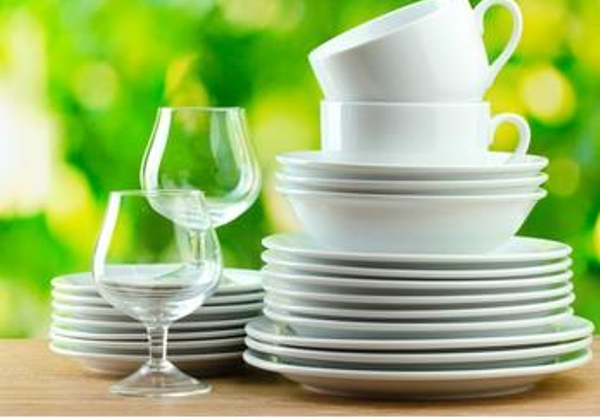
\includegraphics[width=0.32\linewidth]{mucca_mcac_12.png} &
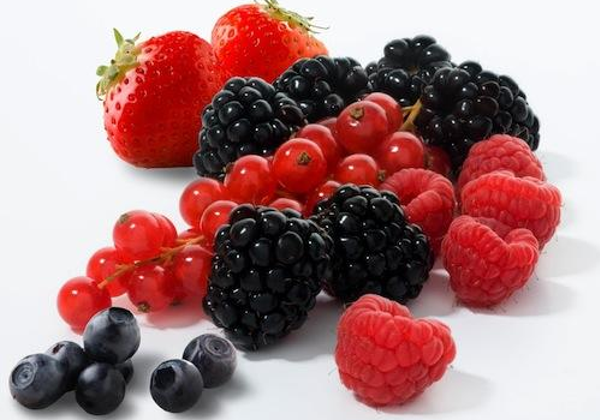
\includegraphics[width=0.32\linewidth]{mucca_mcac_25.png} &
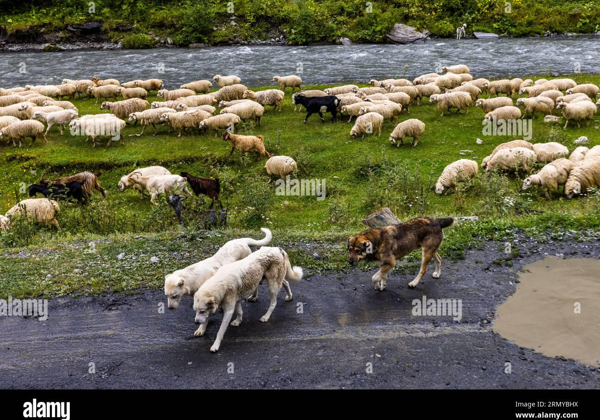
\includegraphics[width=0.32\linewidth]{mucca_mcac_171.png}\\[-0.5mm]
\tiny đĩa--bát & \tiny việt quất--lý chua & \tiny chó--dê\\
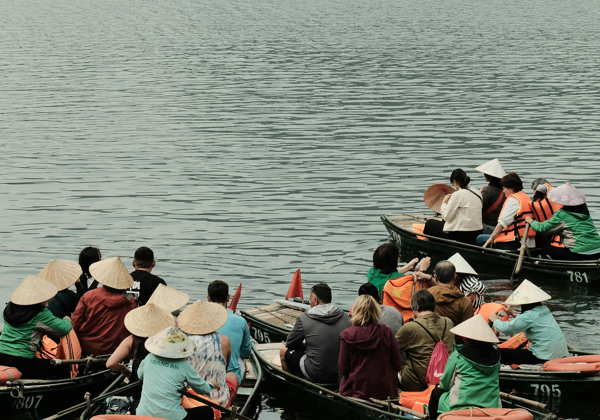
\includegraphics[width=0.32\linewidth]{mucca_mcac_224.png} &
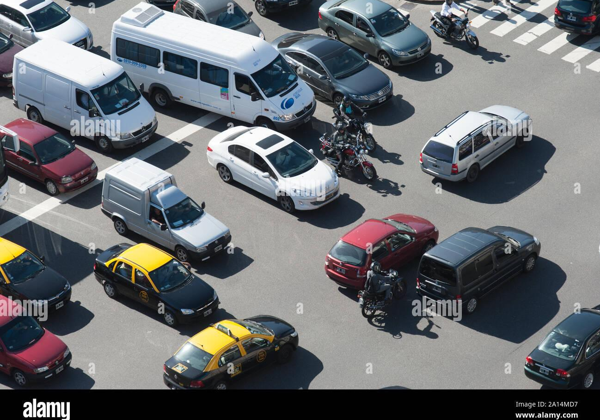
\includegraphics[width=0.32\linewidth]{mucca_mcac_88.png} &
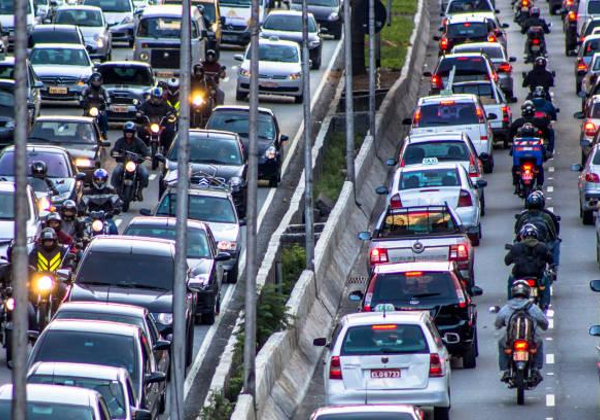
\includegraphics[width=0.32\linewidth]{mucca_mcac_84.png}\\[-0.5mm]
\tiny người--thuyền & \tiny người--ô tô & \tiny người--xe máy
\end{tabular}
\end{column}
\begin{column}{0.52\textwidth}
\small
\begin{tabular}{@{}lll@{}}
\toprule
Tập & Ảnh / query & Dùng để\\
\midrule
Pilot & 5 / 15 & tìm lỗi, làm bản v1\\
p4\_unseen\_v1 & 10 / 30 & kiểm bản v1, blind review N4\\
\textbf{dev v2} & 20 / 60 & chọn cấu hình\\
\textbf{test v2} & 40 / 119 & đo một lần duy nhất\\
\bottomrule
\end{tabular}\\[2mm]
\begin{itemize}\scriptsize
\item Rút mẫu bằng script theo luật cố định, chỉ đọc nhãn; mỗi class có 3--40 vật
\item Lấy hết các cặp khác hẳn nhau (khác nhóm lớn, vd người--xe); phần còn lại là cặp dễ nhầm (cùng nhóm, vd đĩa--bát)
\item Test: 13 ảnh cặp khác hẳn + 27 ảnh cặp dễ nhầm
\item Người kiểm từng ảnh (Trí kiểm dev, Triệu kiểm test), sau đó khóa bằng SHA-256
\end{itemize}
\end{column}
\end{columns}
\note{[0:55] Dữ liệu là MUCCA, 200 ảnh thật, mỗi ảnh nhiều class. Nhóm chia thành bốn tập không trùng nhau. Dev và test được rút bằng script, chỉ đọc nhãn. Cặp khác hẳn nhau như người và xe rất hiếm, chỉ 19 ảnh đủ điều kiện, nên lấy hết; phần còn lại là cặp dễ nhầm như đĩa và bát. Em kiểm từng ảnh test, Trí kiểm dev, rồi khóa bằng hash.}
\end{frame}

\begin{frame}{Giao thức ``chọn trước, xem sau'' và cách đo}
\source{Efron, 1979 (bootstrap); luật D9 trong \texttt{reports/KE\_HOACH\_TIEP\_THEO\_20261105.md}}
\begin{center}
\begin{tikzpicture}[node distance=3mm]
\node[sb=boxgray,text width=20mm] (d) {Dữ liệu được\\người kiểm, khóa};
\node[sb=boxyellow,text width=20mm,right=of d] (r) {Viết trước\\luật chọn \textbf{D9}};
\node[sb=boxblue,text width=20mm,right=of r] (dv) {Chọn trên dev,\\\textbf{khóa} cấu hình};
\node[sb=boxgreen,text width=20mm,right=of dv] (t) {Chạy test\\\textbf{một lần}};
\node[sb=boxgray,text width=20mm,right=of t] (c) {Kiểm hash, tính lại\\từ output thô};
\draw[sa] (d)--(r); \draw[sa] (r)--(dv); \draw[sa] (dv)--(t); \draw[sa] (t)--(c);
\end{tikzpicture}
\end{center}
\begin{columns}[T]
\begin{column}{0.50\textwidth}
\begin{block}{Chỉ số}
\small
$\MAE=\frac{1}{|Q|}\sum_q|\hat n_q-n_q|$ (chỉ số chính)\\[1mm]
$\FPRabs$: tỉ lệ absent query mà mô hình vẫn đếm ra hơn 0\\[1mm]
Shared box X/Y: tỉ lệ box của query này có box trùng (IoU $\ge 0.5$) ở query kia
\end{block}
\end{column}
\begin{column}{0.46\textwidth}
\begin{block}{Luật D9 và CI}
\small
D9: chọn cấu hình có MAE dev nhỏ nhất, \emph{với điều kiện} không kém \Bzero{} ở present query và ở absent query.\\[1mm]
CI 95\%: bootstrap \textbf{theo ảnh} (5000 lần), vì ba query trên cùng một ảnh không độc lập với nhau.
\end{block}
\end{column}
\end{columns}
\note{[1:00] Vì dữ liệu ít mà tham số nhiều, nhóm làm theo kiểu chọn trước, xem sau. Luật chọn D9 được viết trước khi chạy dev: lấy MAE nhỏ nhất, nhưng không được kém B0 ở present query hay absent query. Chọn xong thì khóa lại, rồi em chạy test đúng một lần trên Kaggle. Sau đó trợ lý AI kiểm hash của các file output và tính lại số đếm, MAE từ output thô; kết quả khớp hoàn toàn. CI lấy mẫu lại theo ảnh, vì ba query trên cùng một ảnh không độc lập. Chuyển: phần kết quả, Trí trình bày.}
\end{frame}

\begin{frame}{Kết quả dev: luật D9 chọn P($\tau$ 0.20, $M$ 5) + F}
\source{Dev v2: 20 ảnh, 60 query; khoảng 90 cấu hình}
\begin{columns}[T]
\begin{column}{0.52\textwidth}
\centering\small
\begin{tabular}{@{}lrrr@{}}
\toprule
Cách & MAE $\downarrow$ & MAE present $\downarrow$ & $\FPRabs$ $\downarrow$\\
\midrule
\Bzero & 6.28 & 8.25 & 0.20\\
\Btwo & 9.15 & 12.00 & 0.20\\
\textbf{P(0.20, 5)+F} & \textbf{3.53} & 5.05 & \textbf{0.05}\\
\BtwoF & 3.73 & 5.15 & 0.20\\
P+T+F & 3.78 & -- & --\\
\Csix & 4.02 & 5.80 & 0.05\\
\bottomrule
\end{tabular}
\end{column}
\begin{column}{0.44\textwidth}
\begin{itemize}\small
\item Cấu hình thắng theo D9 được khóa vào file freeze (có hash)
\item Các cấu hình đứng đầu rất sát nhau: 7 họ đầu chỉ cách nhau 0.49 MAE
\item Threshold được chọn ngay trên dev $\Rightarrow$ số dev \alert{lạc quan}
\end{itemize}
\end{column}
\end{columns}
\takeaway{Dev chỉ dùng để chọn; số để báo cáo là số test.}
\note{[0:40] Trên dev, theo luật D9, cấu hình được chọn là P với tau 0.20, M bằng 5, cộng F, MAE 3.53. Các cách đứng đầu rất sát nhau, và threshold được chọn ngay trên dev, nên số này lạc quan. Số để báo cáo là số test.}
\end{frame}

\begin{frame}{Kết quả test: giảm 24\% sai số so với CountGD++ một lượt}
\source{Test v2: 40 ảnh, 119 query (79 present, 40 absent); chạy một lần trên Kaggle T4}
\begin{columns}[c]
\begin{column}{0.48\textwidth}
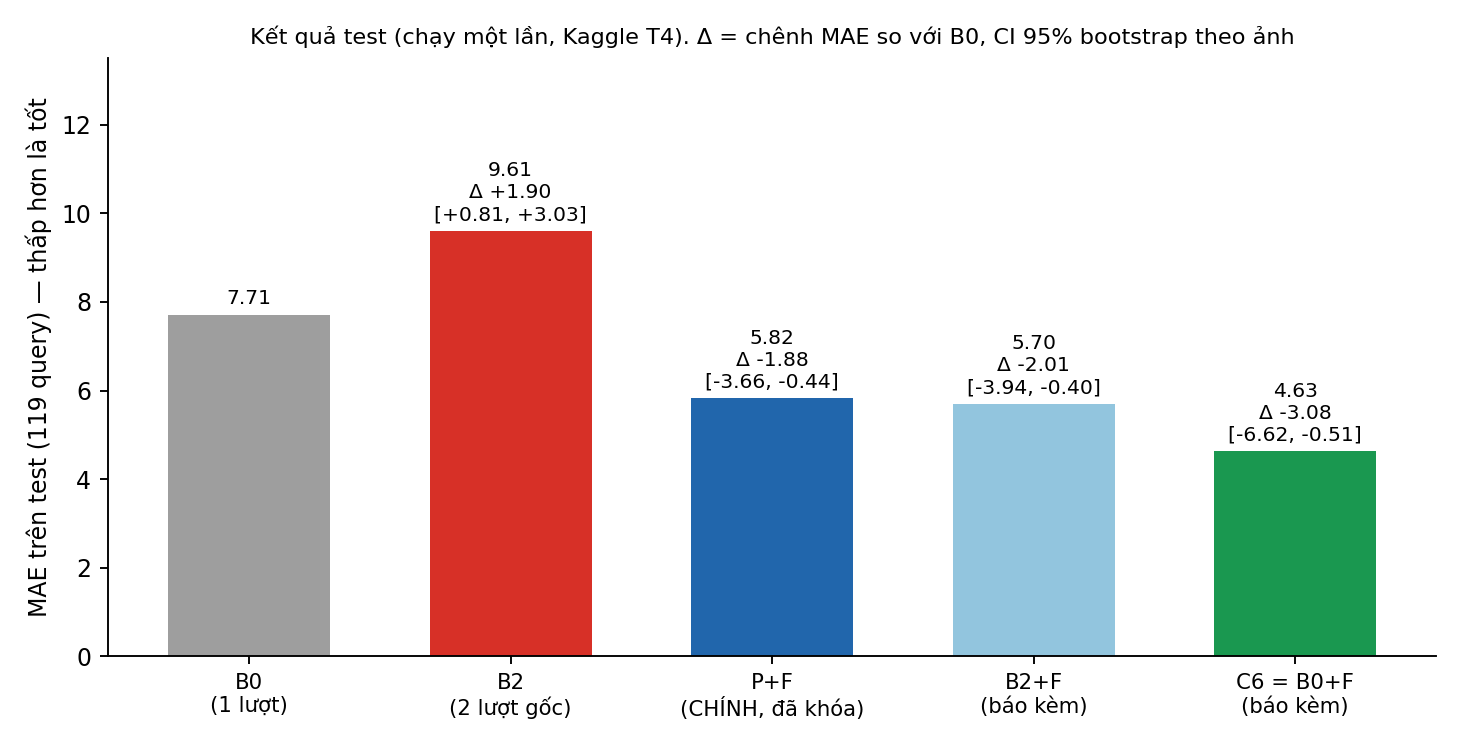
\includegraphics[width=\linewidth]{fig_results_test.png}
\end{column}
\begin{column}{0.50\textwidth}
\centering\small
\begin{tabular}{@{}lrrl@{}}
\toprule
Cách & MAE & $\FPRabs$ & $\Delta$ so với \Bzero{} [CI 95\%]\\
\midrule
\Bzero & 7.71 & 0.250 & --\\
\Btwo & 9.61 & 0.250 & \alert{$+1.90$} [$+0.81$, $+3.03$]\\
\textbf{\PF} & \textbf{5.82} & \textbf{0.225} & $\mathbf{-1.88}$ [$-3.66$, $-0.44$]\\
\BtwoF & 5.70 & 0.250 & $-2.01$ [$-3.94$, $-0.40$]\\
\Csix & 4.63 & 0.100 & $-3.08$ [$-6.62$, $-0.51$]\\
\bottomrule
\end{tabular}\\[2mm]
\begin{itemize}\scriptsize
\item \textbf{RQ3:} cấu hình đã khóa giảm MAE 7.71 $\to$ 5.82, CI không chứa 0
\item Lượt 2 gốc làm kết quả \emph{kém đi}, CI không chứa 0
\item \BtwoF, \Csix: đối chứng khai báo trước, không đổi thành phương pháp chính sau khi xem test
\end{itemize}
\end{column}
\end{columns}
\note{[1:10] Trên 40 ảnh test chưa từng dùng, CountGD++ một lượt có MAE 7.71, tức trung bình sai gần 8 vật mỗi query. Cấu hình đã khóa còn 5.82, giảm 24 phần trăm, CI không chứa 0. Lượt 2 gốc còn tệ hơn một lượt, 9.61, và chênh lệch này cũng đáng tin. Hai dòng dưới là đối chứng khai báo trước; nhóm không đổi chúng thành kết quả chính sau khi xem test. Chuyển: vì sao có mức giảm này, Triệu phân tích.}
\end{frame}

\begin{frame}{Phân rã: cải thiện đến từ filter F, không đến từ P}
\source{Phân tích post-hoc trên test, không dùng để chọn hay đổi phương pháp}
\begin{columns}[T]
\begin{column}{0.48\textwidth}
\begin{block}{P gần như không thay đổi exemplar}
\small
\begin{itemize}
\item Ở \bignum{108/120} query, P chọn đúng bộ pseudo-exemplar như \Btwo
\item Threshold $\tau=0.20$ khá thấp, nên ba box đầu thường đều lọt qua
\item \BtwoF{} so với \PF: $-0.13$ [$-0.41$, $+0.18$], gần như bằng nhau
\end{itemize}
\end{block}
\end{column}
\begin{column}{0.48\textwidth}
\begin{block}{F giảm mạnh đếm thừa, nhưng tăng đếm thiếu}
\centering\small
\begin{tabular}{@{}lrr@{}}
\toprule
79 present query & Tổng đếm thừa & Tổng đếm thiếu\\
\midrule
\Bzero & $+580$ & $-77$\\
\Btwo & $+751$ & $-58$\\
\PF & $+243$ & \alert{$-297$}\\
\bottomrule
\end{tabular}\\[1mm]
\raggedright\scriptsize F bỏ những box mô hình không chắc, trong đó có cả vật đúng.
\end{block}
\end{column}
\end{columns}
\takeaway{Thành phần có tác dụng là F. P đi đúng hướng nhưng threshold quá dễ, nên hầu như không đổi được exemplar.}
\note{[0:55] Phân tích post-hoc trên test cho thấy P gần như luôn chọn lại đúng bộ pseudo-exemplar cũ, 108 trên 120 query, nên B2 cộng F gần bằng P cộng F. Vậy phần có tác dụng là filter F. F giảm mạnh đếm thừa, từ 580 xuống 243, nhưng đếm thiếu tăng từ 77 lên 297, vì filter bỏ cả một số vật đúng.}
\end{frame}

\begin{frame}{F bỏ được box không chứa vật, nhưng chưa tách hẳn X với Y}
\source{Kiểm theo điểm nhãn MUCCA (79 present query); shared box trên 39 ảnh, CI 95\%}
\centering\small
\begin{tabular}{@{}lrrrrl@{}}
\toprule
Cách & Box giữ & Đúng class $\uparrow$ & Class khác $\downarrow$ & Không trúng $\downarrow$ & Shared box X/Y $\downarrow$\\
\midrule
\Bzero & 1481 & 60.4\% & 34.6\% & 5.1\% & 64\% [51, 75]\\
\Btwo & 1671 & 56.6\% & 34.6\% & 8.8\% & 71\% [58, 81]\\
\PF & 924 & 66.3\% & 32.7\% & \textbf{1.0\%} & 59\% [40, 74]\\
\Csix & 746 & \textbf{76.9\%} & \textbf{21.3\%} & 1.7\% & \textbf{24\%} [11, 37]\\
\bottomrule
\end{tabular}\\[3mm]
\begin{columns}[T]
\begin{column}{0.46\textwidth}
\begin{itemize}\small
\item Áp sau lượt 2, F chủ yếu bỏ các box không chứa vật (8.8\% $\to$ 1.0\%)
\item Nhưng vẫn khoảng 1/3 số box nằm trên vật class khác
\end{itemize}
\end{column}
\begin{column}{0.46\textwidth}
\begin{itemize}\small
\item Lọc ngay sau lượt 1 (\Csix) tách tốt hơn: 24\% shared box, 21\% box sai class
\item Cách kiểm ``box có chứa điểm nhãn'' khá dễ dãi, nên tỉ lệ đúng class chỉ là mức trên
\end{itemize}
\end{column}
\end{columns}
\note{[0:50] Xét từng box theo điểm nhãn: áp sau lượt 2, F chủ yếu bỏ các box không chứa vật, từ 8.8 xuống 1 phần trăm, nhưng vẫn khoảng một phần ba số box nằm trên vật class khác, và 59 phần trăm vẫn là shared box. Lọc ngay sau lượt 1, tức C6, tách tốt hơn nhiều.}
\end{frame}

\begin{frame}{Theo loại cặp: cải thiện rõ ở cặp dễ nhầm, chưa rõ ở cặp khác hẳn}
\source{Phân tích post-hoc; nhóm cặp khác hẳn chỉ có 13 ảnh}
\begin{columns}[c]
\begin{column}{0.50\textwidth}
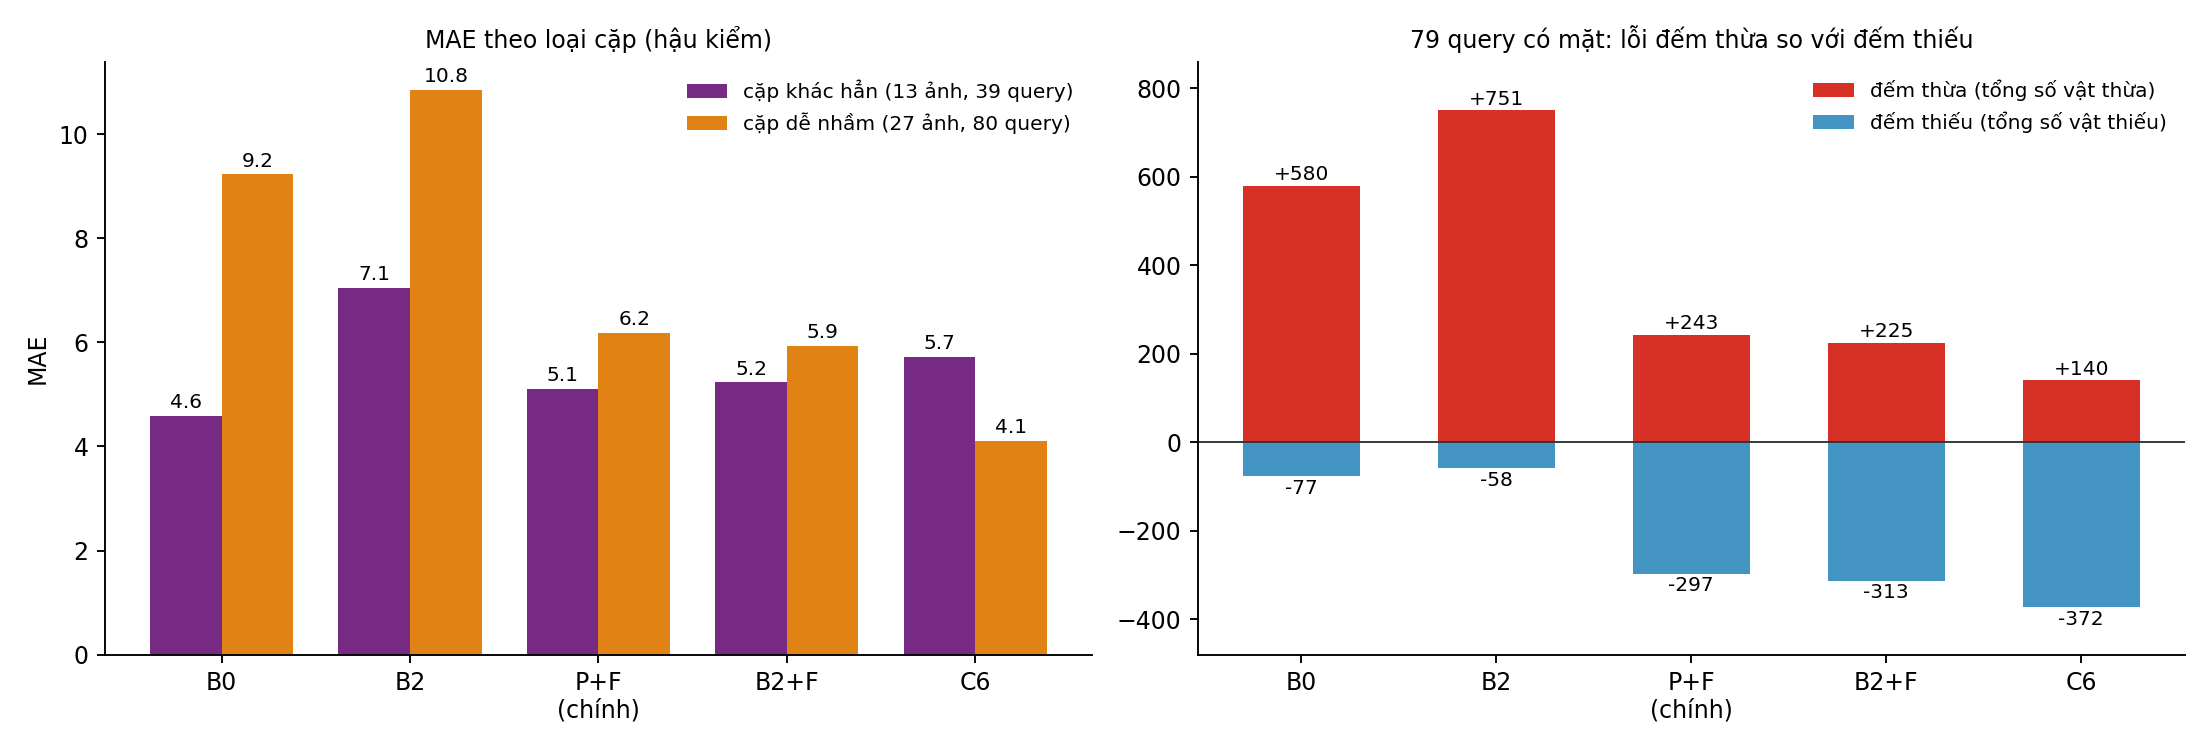
\includegraphics[width=\linewidth]{fig_strata_errors.png}
\end{column}
\begin{column}{0.48\textwidth}
\centering\scriptsize
\begin{tabular}{@{}lll@{}}
\toprule
$\Delta$ MAE so với \Bzero & Khác hẳn (13) & Dễ nhầm (27)\\
\midrule
\Btwo & $+2.46$ [$+0.38$, $+4.74$] & $+1.63$ [$+0.39$, $+2.86$]\\
\PF & $+0.51$ [$-0.72$, $+1.82$] & $\mathbf{-3.05}$ [$-5.43$, $-0.96$]\\
\Csix & $+1.13$ [$-0.87$, $+3.51$] & $\mathbf{-5.13}$ [$-10.16$, $-1.60$]\\
\bottomrule
\end{tabular}\\[2mm]
\begin{itemize}\scriptsize
\item \textbf{Cặp dễ nhầm} (quả với quả, bát với đĩa): \Bzero{} đếm thừa nhiều, nên filter phát huy tác dụng
\item \textbf{Cặp khác hẳn} (người với xe): \Bzero{} vốn đã khá tốt (MAE 4.59); filter lại có xu hướng làm đếm thiếu
\end{itemize}
\end{column}
\end{columns}
\takeaway{Phương pháp chưa giải quyết được mọi dạng X/Y.}
\note{[0:50] Chia theo loại cặp: với cặp dễ nhầm, P cộng F giảm khoảng 3 vật mỗi query, CI không chứa 0. Với cặp khác hẳn, đúng dạng người và xe mà thầy nêu, chưa thấy khác biệt chắc chắn, và nhóm này chỉ có 13 ảnh. Nhóm nói thẳng: phương pháp chưa giải quyết được mọi dạng X/Y.}
\end{frame}

\begin{frame}{Ví dụ: một trường hợp thành công và một lỗi X/Y còn sót}
\source{Xanh: box trúng đúng class · đỏ: chỉ trúng class khác · xám: không trúng điểm nhãn nào}
\centering
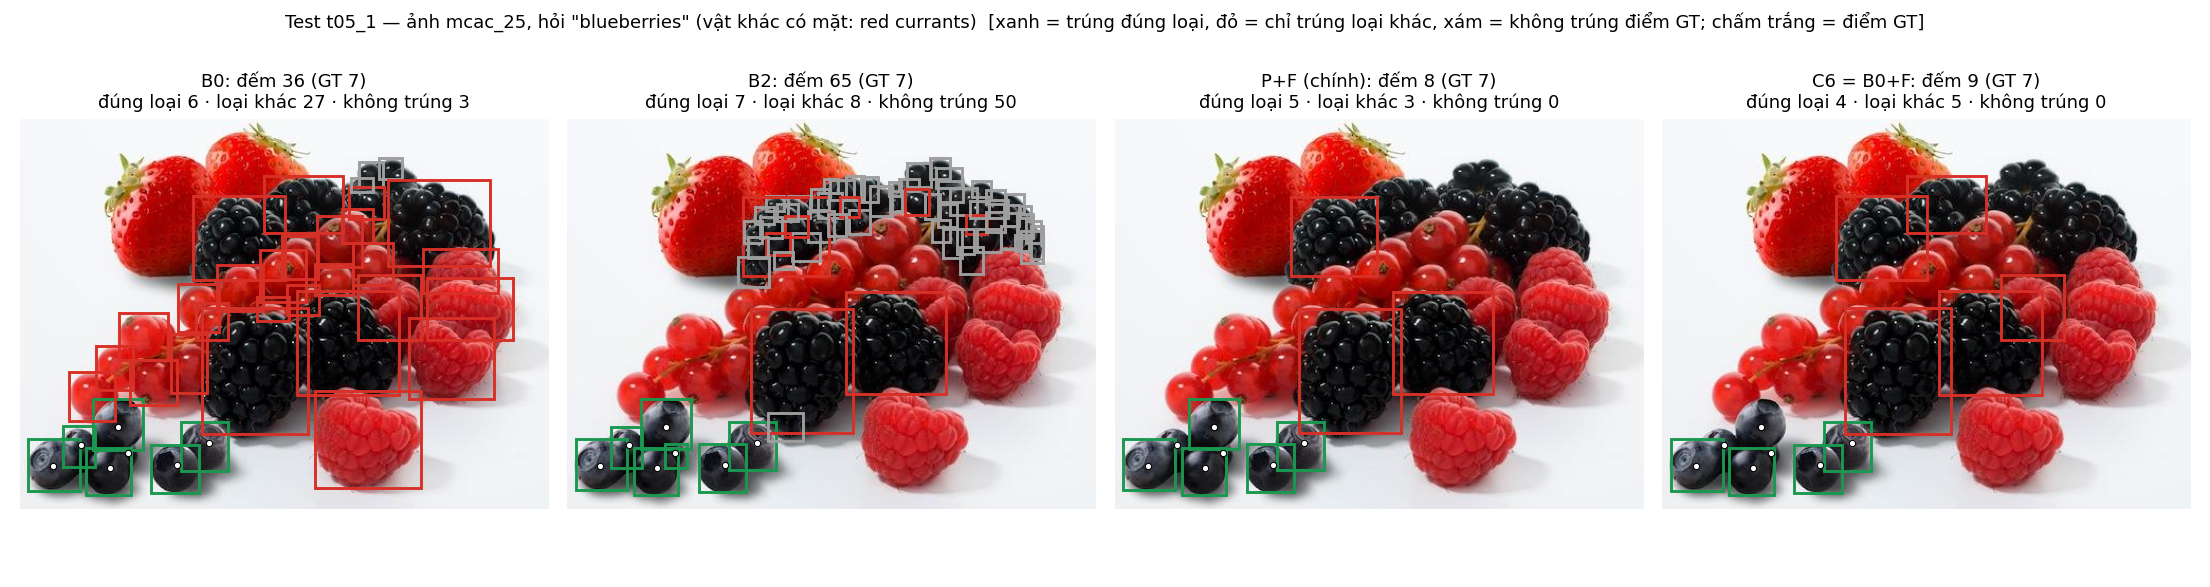
\includegraphics[width=0.80\textwidth]{fig_example_t05_1_mcac_25.png}\\[-0.5mm]
{\scriptsize\textcolor{good}{\textbf{Thành công}} ``blueberries'' (GT 7): \Bzero{} 36 · \Btwo{} 65 · \PF{} \textbf{8} · \Csix{} 9}\\[1mm]
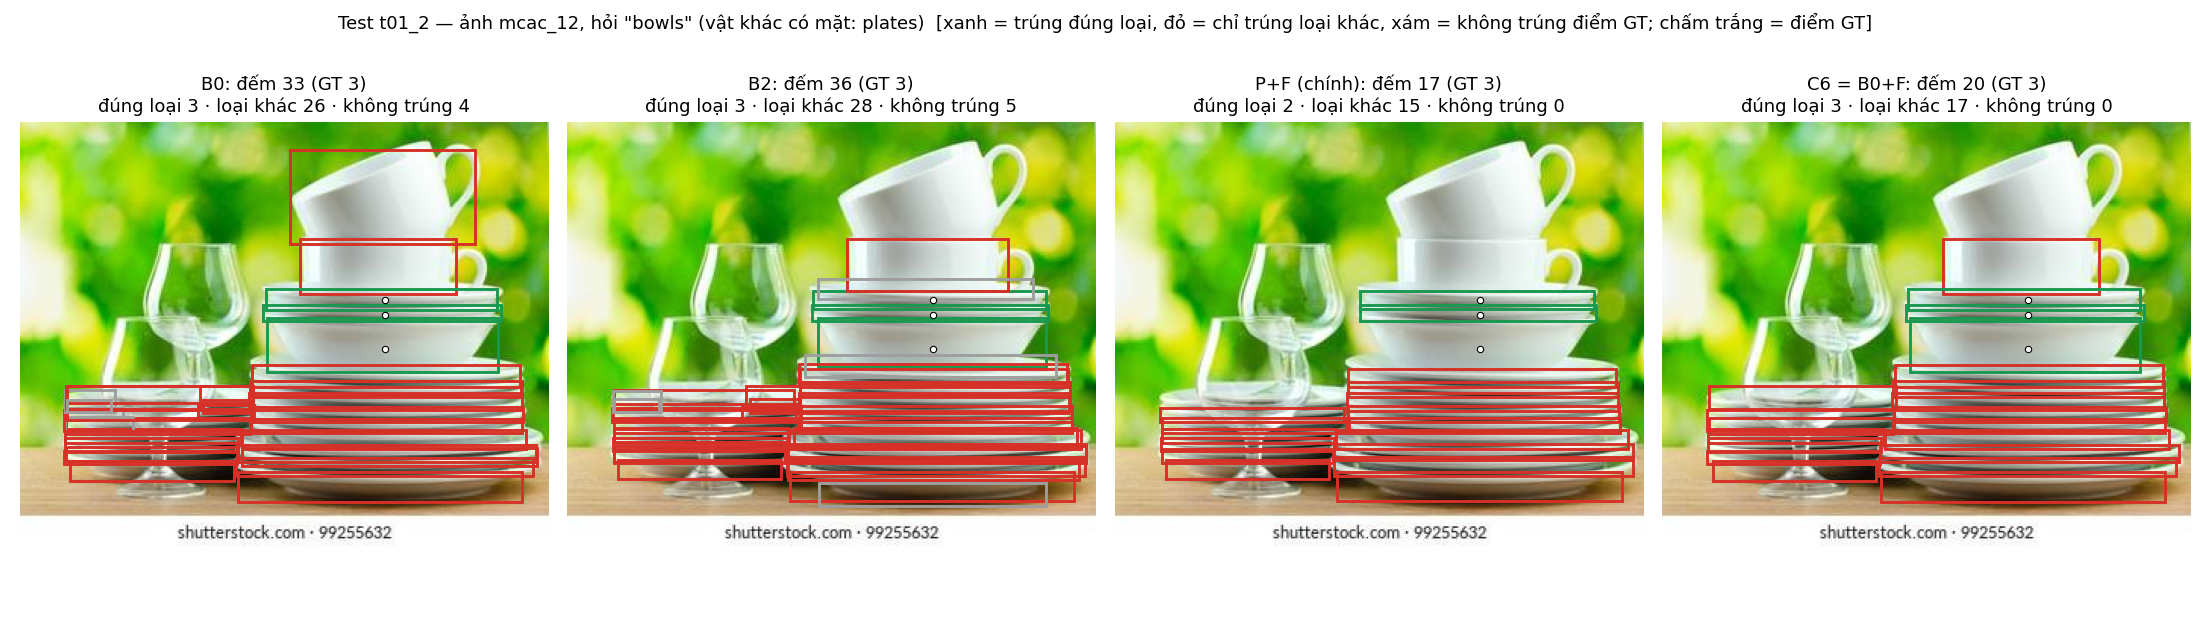
\includegraphics[width=0.80\textwidth]{fig_example_t01_2_mcac_12.png}\\[-0.5mm]
{\scriptsize\textcolor{bad}{\textbf{Lỗi còn sót}} ``bowls'' (GT 3): chồng đĩa vẫn bị đếm là bát ở mọi cách (\PF{} 17, \Csix{} 20)}
\note{[0:45] Ví dụ thành công: blueberries, B2 đếm 65 vì khoanh cả từng hạt của quả mâm xôi đen, còn P cộng F đếm 8, GT là 7. Ví dụ lỗi còn sót: bowls, chồng đĩa vẫn bị đếm là bát ở mọi cách.}
\end{frame}

\begin{frame}{Ví dụ thất bại: CLIP nhầm các class gần giống nhau, và lọc quá tay}
\centering
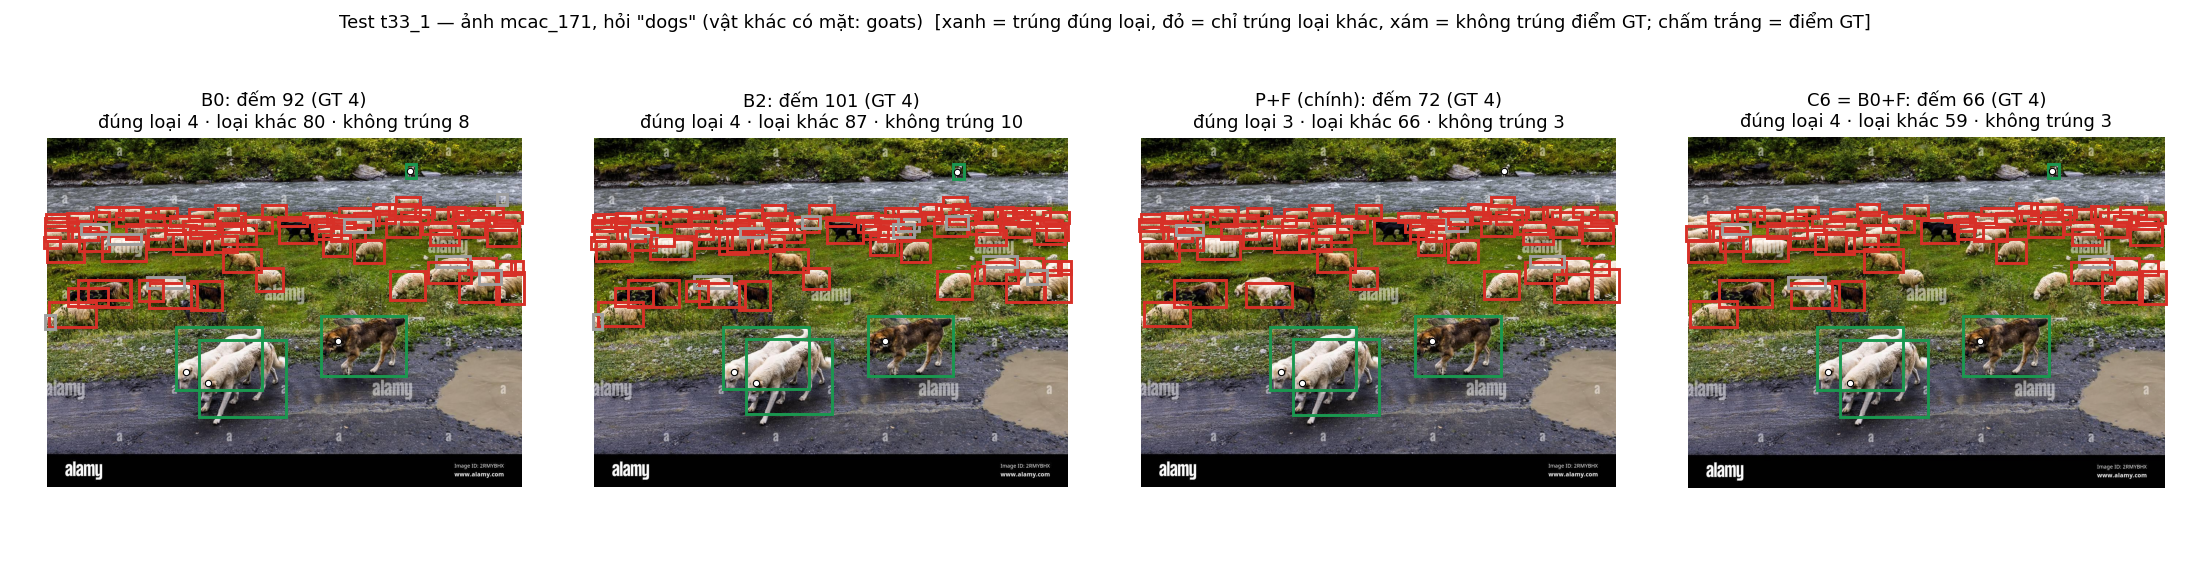
\includegraphics[width=0.80\textwidth]{fig_example_t33_1_mcac_171.png}\\[-0.5mm]
{\scriptsize\textcolor{bad}{\textbf{Nhầm class}} ``dogs'' (GT 4): đàn cừu (cùng vài con dê) bị đếm là chó ở mọi cách (66--101). Trên ô cắt nhỏ, CLIP không phân biệt được cừu, dê với chó.}\\[1mm]
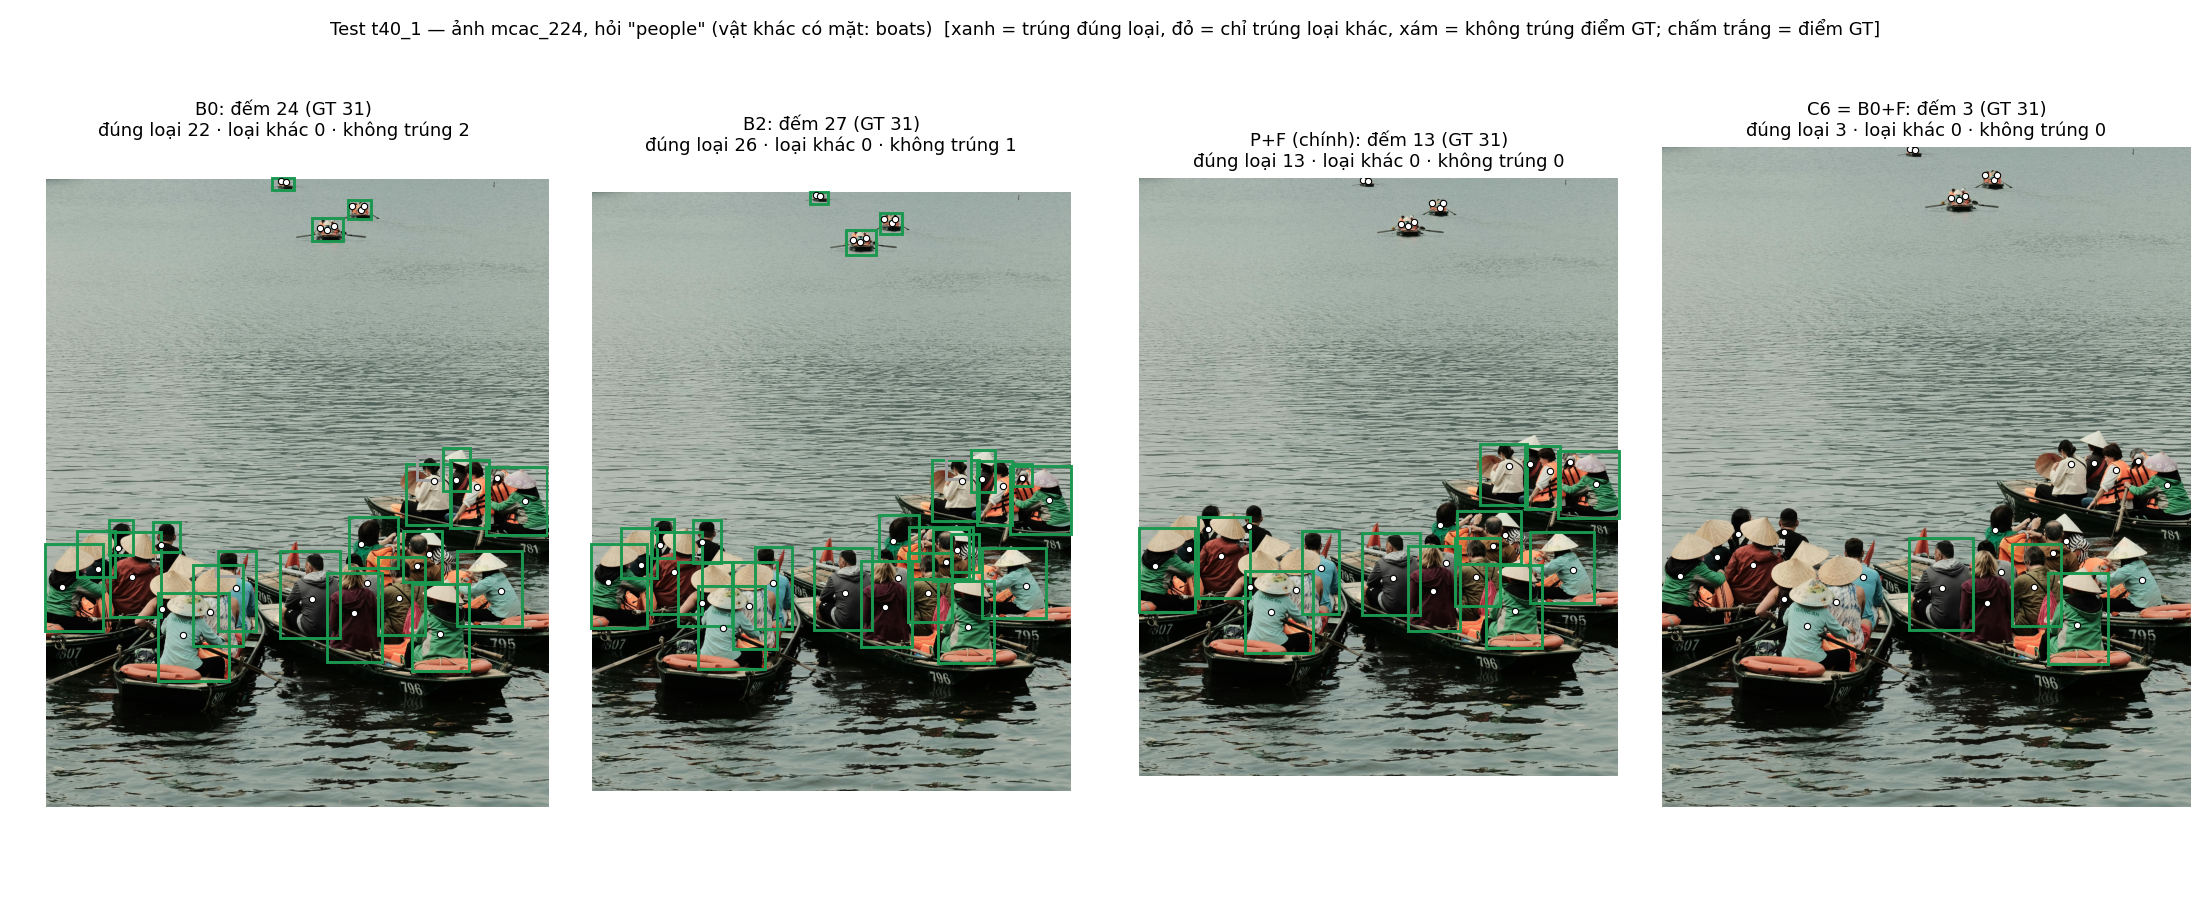
\includegraphics[width=0.54\textwidth]{fig_example_t40_1_mcac_224.png}\\[-0.5mm]
{\scriptsize\textcolor{bad}{\textbf{Lọc quá tay}} ``people'' (GT 31): không có box nào sai class, nhưng F bỏ cả người thật (\PF{} còn 13, \Csix{} còn 3)}
\note{[0:45] Hai kiểu thất bại. Dogs: ảnh có 80 con cừu, 7 con dê và 4 con chó; đàn cừu bị đếm là chó ở mọi cách, vì trên ô cắt nhỏ CLIP cũng không phân biệt được cừu, dê với chó. People: không có box nào sai class, nhưng filter bỏ cả người thật, chỉ còn 13 trên 31.}
\end{frame}

\begin{frame}{Kiểm thêm trên 300 ảnh FSC-147 (mỗi ảnh một class)}
\source{Pre-registered 20/11; chạy một lần trên Kaggle T4; không crop, không exemplar GPT-5; kiểm độc lập PASS}
\begin{columns}[T]
\begin{column}{0.52\textwidth}
\centering\small
\begin{tabular}{@{}lrrrr@{}}
\toprule
Cách & MAE $\downarrow$ & Bias & $\le$40 vật & $>$40 vật\\
\midrule
\Bzero & 13.88 & $-1.54$ & 3.95 & 25.69\\
\Btwo & \textbf{13.32} & $-0.23$ & \textbf{3.44} & \textbf{25.09}\\
\PF & 18.01 & $-14.68$ & 3.50 & \alert{35.28}\\
\BtwoF & 17.98 & $-14.79$ & 3.65 & 35.02\\
\Csix & 25.11 & $-20.93$ & 5.34 & \alert{48.64}\\
\bottomrule
\end{tabular}\\[1mm]
\raggedright\scriptsize Không so với 8.34 / 8.39 vì khác điều kiện (có crop, có exemplar GPT-5, đủ 1.190 ảnh).
\end{column}
\begin{column}{0.44\textwidth}
\begin{itemize}\small
\item \textbf{So sánh chính} \Bzero{} $-$ \Btwo: $+0.55$ [$-3.00$, $+4.30$] $\Rightarrow$ với ảnh một class, giữ hay bỏ lượt 2 \emph{chưa khác nhau rõ}
\item \PF{} $-$ \Btwo: \alert{$+4.69$} [$+2.25$, $+7.50$] $\Rightarrow$ cấu hình của nhóm kém hơn
\item Kém chủ yếu ở ảnh trên 40 vật, do \textbf{đếm thiếu} (thiếu 4416 vật, so với 1910 của \Btwo)
\item Có thể do threshold của F được chọn trên ảnh 3--40 vật; chưa tách được ảnh hưởng của density với khác biệt giữa hai bộ dữ liệu
\end{itemize}
\end{column}
\end{columns}
\takeaway{Cải tiến phù hợp với ảnh nhiều class, số vật ít đến vừa. Với ảnh một class, nhiều vật, nên giữ CountGD++ gốc.}
\note{[0:55] Em chạy thêm một khảo sát pre-registered trên 300 ảnh FSC-147, mỗi ảnh một class. Giữ hay bỏ lượt 2 chưa khác nhau rõ, nên kết luận lượt 2 gây hại chỉ đúng cho ảnh nhiều class. Cấu hình của nhóm kém hơn, chủ yếu ở ảnh trên 40 vật, và lỗi là đếm thiếu. Một giải thích có thể là threshold của F được chọn trên ảnh ít vật nên lọc quá tay, nhưng khảo sát chưa tách được ảnh hưởng của density với khác biệt giữa hai bộ dữ liệu. Ở ảnh tối đa 40 vật thì hai cách gần nhau.}
\end{frame}

\begin{frame}{Các hướng đã thử thêm (chỉ trên dev)}
\source{Pre-registered 22/11, không chạy trên test; dev đã dùng để chọn F nên kết quả chỉ là sơ bộ}
\begin{columns}[T]
\begin{column}{0.52\textwidth}
\begin{block}{Gán mỗi box cho class giống nhất (bước A)}
\small Mỗi box được CLIP so với mọi class được hỏi trên ảnh (X, Y, Z); chỉ giữ box nếu nó giống class đang hỏi nhất. Bước này không có tham số nào.\\[1mm]
\centering
\begin{tabular}{@{}lrr@{}}
\toprule
Dev & \PF & + bước A\\
\midrule
Shared box X/Y $\downarrow$ & 61.6\% & \textbf{2.9\%}\\
Box đúng class $\uparrow$ & 70.2\% & 83.0\%\\
MAE present query $\downarrow$ & \textbf{5.05} & 6.92\\
\bottomrule
\end{tabular}\\[1mm]
\raggedright\scriptsize So sánh chính: shared box $-0.587$ [$-0.735$, $-0.404$]; MAE $+1.88$ [$-0.03$, $+3.73$] $\Rightarrow$ \textbf{đánh đổi}: CLIP bỏ nhầm khoảng 30\% vật đúng.
\end{block}
\end{column}
\begin{column}{0.44\textwidth}
\begin{alertblock}{Bài học khi chọn cấu hình (\Csix)}
\scriptsize
\begin{tabular}{@{}lrrr@{}}
\toprule
Cách & Dev & Test & Thay đổi\\
\midrule
\Bzero & 6.28 & 7.71 & $+1.42$\\
\PF{} (thắng theo D9) & 3.53 & 5.82 & $+2.29$\\
\Csix & 4.02 & 4.63 & $+0.61$\\
\bottomrule
\end{tabular}\\[1mm]
\small Chênh lệch giữa các cách nằm trong sai số ở cả dev lẫn test; cách thắng trên dev lại tăng sai số nhiều nhất khi sang test. Nhóm \textbf{không đổi} kết quả chính sau khi đã xem test.
\end{alertblock}
\end{column}
\end{columns}
\note{[1:00] Nhóm thử thêm một hướng nhắm thẳng vào bài X/Y: gán mỗi box cho class mà CLIP thấy giống nhất. Shared box giảm từ 62 xuống 3 phần trăm, nhưng CLIP trên ô cắt nhỏ bỏ nhầm khoảng 30 phần trăm vật đúng, nên số đếm chưa tốt hơn. Bài học thứ hai: trên dev, C6 chỉ đứng thứ 7 trong 15 họ cấu hình, nhưng lại tốt nhất trên test; chênh lệch nằm trong sai số, nên nhóm không đổi kết quả chính sau khi đã xem test.}
\end{frame}

% ================================================================ 5
\section{Giới hạn và kết luận}

\begin{frame}{Những điều kết quả này chưa trả lời được}
\begin{columns}[T]
\begin{column}{0.48\textwidth}
\textbf{Về phương pháp}
\begin{itemize}\small
\item Bài X/Y \textbf{chưa giải quyết xong}: MAE present query vẫn là 6.84, trong khi mỗi query trung bình chỉ có 12.4 vật; 59\% box vẫn là shared box
\item Filter F dùng một threshold chung cho mọi ảnh, nên lọc quá tay ở ảnh đông vật
\item CLIP yếu với ô cắt nhỏ và các class gần giống nhau (cừu/dê--chó, chồng đĩa--bát)
\item Cơ chế của lượt 2: giả thuyết H2 chưa kiểm; chưa chạy \Tv{} trên test
\end{itemize}
\end{column}
\begin{column}{0.48\textwidth}
\textbf{Về cách đánh giá}
\begin{itemize}\small
\item Test chỉ có 40 ảnh, trong đó 13 ảnh cặp khác hẳn; phân tích theo nhóm là post-hoc
\item Kết quả chính chỉ trên một bộ dữ liệu (MUCCA)
\item 15/120 query test có ghi chú cần xem lại nhãn (thay bằng số người đếm thì MAE đổi dưới 0.06)
\item Chưa đo riêng thời gian CLIP của từng cấu hình
\end{itemize}
\end{column}
\end{columns}
\takeaway{Nhóm không gọi đây là SOTA: cải thiện có phạm vi, có điều kiện, và kèm xu hướng đếm thiếu.}
\note{[0:50] Nhóm tự nêu những điều kết quả chưa trả lời được. Về phương pháp: bài X/Y chưa giải quyết xong, threshold dùng chung cho mọi ảnh, CLIP yếu với các class gần giống nhau, giả thuyết H2 chưa kiểm. Về đánh giá: mẫu nhỏ, chỉ một bộ dữ liệu, một số nhãn cần xem lại. Chuyển: Trí tóm tắt kết luận.}
\end{frame}

\begin{frame}{Kết luận: vấn đề, cải tiến và kết quả}
\small
\begin{tabularx}{\textwidth}{@{}l l X@{}}
\toprule
Vấn đề (RQ1) & Cải tiến (RQ2) & Kết quả (RQ3, test khóa trước)\\
\midrule
VĐ1. Đổi query, box gần như không đổi & \textbf{F}: CLIP kiểm từng box & \textcolor{good}{\ding{51}} \PF: 7.71 $\to$ \textbf{5.82} ($-24\%$, CI không chứa 0); chủ yếu ở cặp dễ nhầm\\
VĐ2. Pseudo-exemplar sai class & \textbf{P}: CLIP kiểm pseudo-exemplar & \textcolor{bad}{\ding{55}} hầu như không đổi exemplar (108/120 query giống \Btwo)\\
VĐ3. Lượt 2 làm lỗi nặng thêm & \textbf{T}: bỏ phép $\max$ (phép thử) & một phần: gỡ 21\% tác hại trên dev; \Btwo{} kém \Bzero{} trên test\\
\midrule
Phạm vi & FSC-147, 300 ảnh & \textcolor{bad}{\ding{55}} kém CountGD++ gốc ở ảnh dày ($+4.69$) $\Rightarrow$ dùng cho ảnh nhiều class, ít đến vừa vật\\
\bottomrule
\end{tabularx}
\takeaway{Sửa ở bước suy luận giảm được lỗi đếm nhầm class, nhưng bài X/Y mới giảm được một phần, chưa giải quyết xong.}
\note{[1:00] Tóm lại: CountGD++ đếm lẫn class trên ảnh nhiều class, và lượt 2 làm lỗi nặng thêm. Filter F dùng CLIP, không cần huấn luyện, giảm 24 phần trăm sai số trên tập test khóa trước. P gần như không đóng góp; phép max chỉ giải thích một phần. Cải tiến dành cho ảnh nhiều class, số vật ít đến vừa.}
\end{frame}

\begin{frame}{Hướng phát triển}
\begin{enumerate}
\item \textbf{Chỉ phân xử những box bị X và Y tranh nhau} bằng CLIP, giữ nguyên các box khác; dùng verifier mạnh hơn (CLIP lớn hơn, crop có thêm ngữ cảnh)
\item \textbf{Threshold thích ứng theo density}, để tránh đếm thiếu ở ảnh dày
\item \textbf{Kiểm \Csix} (lọc ngay sau lượt 1) trên một tập mới, độc lập
\item \textbf{Kiểm giả thuyết H2}: so text score của cùng một box ở lượt 1 và lượt 2
\item Dùng negative prompt ``không đếm Y'' có sẵn trong CountGD++ khi hỏi X
\end{enumerate}
\vspace{2mm}
{\small Mọi hướng trên đều cần một tập kiểm mới, vì tập test hiện tại đã dùng một lần.}
\note{[0:30] Các hướng tiếp theo: chỉ phân xử những box bị tranh chấp, threshold theo density, kiểm C6 và giả thuyết H2 trên dữ liệu mới.}
\end{frame}

\begin{frame}[standout]
Cảm ơn thầy và các bạn đã lắng nghe!\\[4mm]
{\normalsize Mã nguồn, dữ liệu khóa và kết quả:}\\
{\small\url{https://github.com/minhtridaoo/zero-shot-counting}}
\note{Em cảm ơn thầy và các bạn. Nhóm sẵn sàng nhận câu hỏi. Nếu thầy muốn xem thêm, nhóm có slide dự phòng và demo tĩnh bằng các hình ví dụ.}
\end{frame}

% ================================================================ Backup
\appendix
\section*{Slide dự phòng}

\begin{frame}{Dự phòng · Kết quả test đầy đủ}
\small\centering
\begin{tabular}{@{}lrrrrl@{}}
\toprule
Cách & MAE & RMSE & MAE present & $\FPRabs$ & $\Delta$ so với \Bzero{} [CI 95\%]\\
\midrule
\Bzero & 7.71 & 16.63 & 8.32 & 0.250 & --\\
\Btwo & 9.61 & 19.87 & 10.24 & 0.250 & $+1.90$ [$+0.81$, $+3.03$]\\
\textbf{\PF} & \textbf{5.82} & 12.11 & 6.84 & 0.225 & $-1.88$ [$-3.66$, $-0.44$]\\
\BtwoF & 5.70 & 11.85 & 6.81 & 0.250 & $-2.01$ [$-3.94$, $-0.40$]\\
\Csix & 4.63 & 9.63 & 6.48 & 0.100 & $-3.08$ [$-6.62$, $-0.51$]\\
\bottomrule
\end{tabular}\\[3mm]
\raggedright
\begin{itemize}\small
\item \Csix{} $-$ \PF: $-1.19$ [$-3.32$, $+0.24$], chưa đủ chắc
\item Độ nhạy D11 (thay GT bằng số người đếm): MAE đổi dưới 0.06, thứ tự không đổi
\item So với \Btwo{} giảm 39\%: chỉ là con số mô tả, không nằm trong kiểm định khai báo trước
\end{itemize}
\end{frame}

\begin{frame}{Dự phòng · Cải tiến v1 trên 10 ảnh mới}
\small\centering
\begin{tabular}{@{}lrrrr@{}}
\toprule
p4\_unseen\_v1 (30 query) & MAE & MAE present & Đếm TB ở absent query & Box sai class\\
\midrule
\Bzero & 6.77 & \textbf{5.70} & 8.9 & 106\\
\Btwo & 13.00 & 12.95 & 13.1 & 238\\
\Btwo{} + lọc điểm & 7.27 & 8.75 & 4.3 & 92\\
\Btwo{} + lọc kết hợp & \textbf{5.53} & 7.80 & \textbf{1.0} & \textbf{31}\\
\bottomrule
\end{tabular}\\[3mm]
\raggedright\small Lọc kết hợp chặn absent query tốt nhưng bỏ khoảng nửa vật đúng $\Rightarrow$ bản v2 sửa thêm từ nguồn lỗi (pseudo-exemplar, bước P).
\end{frame}

\begin{frame}{Dự phòng · Chi phí tính toán và tái lập}
\begin{columns}[T]
\begin{column}{0.46\textwidth}
\textbf{Kaggle T4}
\begin{itemize}\small
\item \Bzero: khoảng 0.89 s/query
\item \Btwo, P: khoảng 1.5 s/query (lượt 2 chạy ở khoảng 70\% query)
\item CLIP: chấm box của 3 nguồn mất 404 s / 300 query (FSC-147, ảnh nhiều box); chưa đo riêng từng cấu hình
\item \Csix{} bỏ lượt 2: tiết kiệm khoảng 40\% thời gian CountGD++
\end{itemize}
\end{column}
\begin{column}{0.50\textwidth}
\textbf{Tái lập}
\begin{itemize}\small
\item Dữ liệu dev/test \texttt{LOCKED} kèm SHA-256
\item Cấu hình khóa: \texttt{freeze\_v2\_20261111.json} (sha \texttt{64e89ef5\ldots})
\item Kiểm A: lượt 1 của P trùng \Bzero; Kiểm C: \Btwo{} chạy lại trùng 60/60
\item Kết quả được kiểm hash và tính lại từ output thô, khớp tuyệt đối
\end{itemize}
\end{column}
\end{columns}
\end{frame}

\begin{frame}{Dự phòng · Thứ hạng dev theo họ phương pháp}
\small\centering
\begin{tabular}{@{}rlr@{}}
\toprule
Hạng & Họ (thành viên tốt nhất) & MAE dev\\
\midrule
1 & \PF & 3.53\\
2 & \BtwoF & 3.73\\
3 & P+T+F & 3.78\\
4 & P+S & 3.93\\
5 & T+F & 3.95\\
6 & P+T+S & 3.98\\
7 & \Csix{} (\Bzero+F) & 4.02\\
11 & \Bzero & 6.28\\
15 & \Btwo & 9.15\\
\bottomrule
\end{tabular}\\[2mm]
\raggedright\small 7 họ đầu cách nhau 0.49 MAE, trong khi một CI điển hình rộng khoảng 2: 60 query dev không đủ để phân biệt các cách đứng đầu.
\end{frame}

\end{document}
